% config from Lipics
\documentclass[a4paper,UKenglish]{lipics-v2016}

\usepackage{microtype}%if unwanted, comment out or use option "draft"

%\graphicspath{{./graphics/}}%helpful if your graphic files are in another directory

\bibliographystyle{plainurl}% the recommended bibstyle

\usepackage{latexsym}
\usepackage{mathabx}
\usepackage{float}
\usepackage[scaled]{helvet}
%% \usepackage[noend]{algorithmic}
%% \usepackage{mathrsfs}
%% \usepackage{mathpartir}
%% \usepackage{dsfont}
\usepackage{stmaryrd}
%% \usepackage{textcomp}
%% \usepackage{titlesec}
%% \usepackage{parskip}
\usepackage{alltt}
%% \usepackage{bbm}
%% \usepackage{verbdef}
\usepackage{xspace}
\usepackage{verbatim}
% Enumiten is blacklisted by the .CLS manual
%\usepackage{enumitem}
%\usepackage{lipsum}
\usepackage{wrapfig}
\usepackage[usenames,dvipsnames]{xcolor}
\hypersetup{linkcolor=black,citecolor=black,urlcolor=RubineRed}

\newcounter{tags}
\usepackage{pgf,tikz}  
\usepackage{cite}
% For turned column headers 
%\usepackage{adjustbox} 
%\usepackage{booktabs}
%\usepackage{pifont}
\input{flags}
%%%%%%%%%%%%%%%%%%%%%%%%%%%%%%%%%%%%%%%%%%%%%%%%%%%%%%%%%%%%%%%%%%%%%%
% Compiling two paper versions
%%%%%%%%%%%%%%%%%%%%%%%%%%%%%%%%%%%%%%%%%%%%%%%%%%%%%%%%%%%%%%%%%%%%%%

\newcommand{\ifext}[2]{\ifdefined\extflag{#1}\else{#2}\fi}
\newcommand{\ifcomm}[1]{\ifdefined\extcomm{#1}\else{}\fi}

\newcommand{\mute}[1]{\ifdefined\draftflag{#1} \else{} \fi}
%\newcommand{\mute}[1]{}

\usepackage{skull}

\newcounter{ToDos}
\newcounter{WarnCounts}
\newcommand{\decorateWC}{
  \stepcounter{WarnCounts}
  \marginpar{\textcolor{red}{$\skull\ \theWarnCounts$}}}

\newcommand{\decorateTD}{
  \stepcounter{ToDos}
  \marginpar{\textcolor{red}{$\textbf{TO DO}_{\#\ \theToDos}$}}}


% Skeleton for remark comments
% 1: Name, 2: Color, 3:Comment
\newcommand{\signedComment}[3]
           {\mute{\textcolor{#2}{(#1: {#3})}\decorateWC}}

% remarks
\newcommand{\todo}[1]{\mute{\textcolor{red}{(TO DO:{#1})}\decorateTD}}

\newcommand{\is}[1]{\signedComment{Ilya}{blue}{#1}}
\newcommand{\an}[1]{\signedComment{Aleks}{red}{#1}}
\newcommand{\ab}[1]{\signedComment{AB}{red}{#1}}
\newcommand{\gad}[1]{\signedComment{GAD}{red}{#1}}

\newcommand{\highlight}[1]
           {\ifdefined\draftflag{{\textcolor{red}{#1}}} \else{#1} \fi}

\newenvironment{draft}
           {\ifdefined\draftflag \par\color{red} \else \comment \fi}
           {\ifdefined\draftflag \decorateWC\par \else \endcomment \fi}
           
% useful macros
\newcommand{\asgn}{\leftarrow}
\newcommand{\code}[1]{\lstinline[basicstyle=\small\ttfamily]{#1}}
\newcommand{\ccode}[1]{\lstinline[basicstyle=\footnotesize\ttfamily]{#1}}
\newcommand{\cccode}[1]{\lstinline[basicstyle=\scriptsize\ttfamily]{#1}} 
\newcommand{\Code}[1]{\code{#1}}
\newcommand{\etc}{\emph{etc}}
\newcommand{\ie}{\emph{i.e.}\xspace}
\newcommand{\id}{\emph{Id.}\xspace}
\newcommand{\eg}{\emph{e.g.}\xspace}
\newcommand{\vs}{\emph{vs.}\xspace}
\newcommand{\etal}{\emph{et~al.}\xspace}
\newcommand{\adhoc}{\emph{ad~hoc}\xspace}
\newcommand{\viz}{\emph{viz.}\xspace}
\newcommand{\dom}[1]{\mathsf{dom}(#1)}
\newcommand{\aka}{\textit{a.k.a.}\xspace}
\newcommand{\cf}{\textit{cf.}\xspace}
\newcommand{\wrt}{{wrt.}\xspace}
\newcommand{\Iff}{{iff}\xspace}
\newcommand{\loef}{L\"{o}f}
\newcommand{\sep}{\textasteriskcentered}
\newcommand{\res}{\mathsf{res}}
\newcommand{\bal}{\mathit{bal}} 
\newcommand{\ret}{\mathsf{ret}} 
\newcommand{\fix}{\mathsf{fix}} 
\newcommand{\Unit}{\mathsf{Unit}}  
\newcommand{\ic}{\mathcal{I}}
\newcommand{\Ic}[2]{\ic~{#1}~{#2}}
\newcommand{\hide}{\mathsf{hide}}  
\newcommand{\last}{\mathsf{last}}  

%specs
\newcommand{\specK}[1]{\ensuremath{\textcolor{blue}{#1}}}
\newcommand{\comm}[1]{\ensuremath{\textcolor{gray}{\esc{/\!/}~{#1}}}}
\newcommand{\spec}[1]{\specK{\left\{{#1}\right\}}}
\newcommand{\specQ}[4]{[#1 , #2 , #3] \, #4}%\specQ{mL}{gL}{gE}{p}
\newcommand{\drspec}[1]{\specK{\langle{#1}\rangle}}
\newcommand{\sspec}[1]{\specK{\{{#1}\}}}
\newcommand*{\backin}{\rotatebox[origin=c]{-180}{$\in$}}%

%actions
\newcommand{\act}[1]{\textsf{\small{#1}}}
\newcommand{\aux}[1]{\textit{#1}}
\newcommand{\Aux}[1]{\(\mathit{\small{#1}}\)}
\newcommand{\Num}[1]{{\text{{\scriptsize{#1}}}}}
\newcommand{\esc}[1]{\text{\texttt{\small{#1}}}}
\newcommand{\kw}[1]{\text{\textbf{#1}}}
\newcommand{\tp}[1]{\text{\textsf{#1}}}
\newcommand{\Asgn}{\leftarrow} 

%PCMs
\newcommand{\dotcup}{\ensuremath{\mathaccent\cdot\cup}}
\newcommand{\pcmS}{\mathbb{U}}
\newcommand{\pcmF}{\bullet}
\newcommand{\join}{\pcmF}
\newcommand{\jjoin}[1]{\ensuremath{\bigodot}_{#1=1}^n} 
\newcommand{\pcmU}{\mathbbm{1}}

% Pretty table
\newcommand{\cmark}{\ding{52}}%
\newcommand{\xmark}{\ding{55}}%
\newcommand*\rot{\rotatebox{32}} 
\newcommand{\yep}{\ding{51}}
\newcommand{\yepl}{$\text{\ding{51}}_{\!\!L}$}  
\newcommand{\yepa}{$\text{\ding{51}}_{\!\!L}$}  
\newcommand{\intab}[1]{({\sffamily{\small{#1}}})}

% Concurroids
\newcommand{\acon}{\mathcal{A}}
\newcommand{\econ}{\mathcal{E}}
\newcommand{\ucon}{\mathcal{U}}
\newcommand{\rcon}{\mathcal{R}}
\newcommand{\ccon}{\mathcal{C}}
\newcommand{\vcon}{\mathcal{V}}
\newcommand{\wcon}{\mathcal{W}}
\newcommand{\privcon}{\mathcal{P}}
\newcommand{\pscon}{\mathcal{S}}
\newcommand{\tbcon}{\mathcal{T}}
\newcommand{\fccon}{\mathcal{F}}
\newcommand{\lcon}{\mathcal{L}}
\newcommand{\alloccon}{\mathcal{A}}
\newcommand{\jayanticon}{\mathcal{J}}

%Getters
\newcommand{\lcl}{{\mathsf{s}}}%L
\newcommand{\env}{{\mathsf{o}}}%E
\newcommand{\joint}{{\mathsf{j}}}%E

\newcommand{\selfsub}{\mathsf{s}}
\newcommand{\othersub}{\mathsf{o}}
\newcommand{\jointsub}{\mathsf{j}}

\newcommand{\hist}{\chi} 
\newcommand{\histS}{\hist_{\, \selfsub}}
\newcommand{\histO}{\hist_{\, \othersub}}
\newcommand{\histJ}{\hist_{\, \jointsub}}
\newcommand{\hempty}{\emptyset}
\def\envsteps{\rightarrow^{*}_{\epsilon}}

\newcommand{\heap}{h} 
\newcommand{\heapS}{\heap_{\, \selfsub}}
\newcommand{\heapSP}{\heap_{\, \selfsub}'}

% Jayanti's Snapshot getters

\def\ordlist{\sigma}
\newcommand{\E}{\tau}
\newcommand{\C}{\kappa}


% Jayanti's Snapshot Orders
\newcommand{\tleq}{\mathrel{\leq_\ordlist}}
\newcommand{\tle}{\mathrel{<_\ordlist}}

\newcommand{\stableorder}{\Omega}
\newcommand{\prefix}[1]{-\,{\tleq}\,#1}

% Primed getters

\def\ordlistP{\sigma'}
\newcommand{\stableorderP}{\stableorder'}
\newcommand{\prefixP}[1]{(\mathrel{\tleqP}#1)}
\newcommand{\tleP}{\mathrel{<_\ordlistP}}
\newcommand{\tleqP}{\mathrel{\leq_\ordlistP}}
\newcommand{\EP}{\tau'}
\newcommand{\CP}{\kappa'}
\newcommand{\histP}{\chi'} 
\newcommand{\histSP}{\hist_{\, \selfsub}'}
\newcommand{\histOP}{\hist_{\, \othersub}'}
\newcommand{\histJP}{\hist_{\, \jointsub}'}

\newcommand{\wxP}{W_\x'}
\newcommand{\wyP}{W_\y'}
\newcommand{\wppP}{W_p'}

\newcommand{\jge}{\mathrel{>_\ordlist}}

\def\lgVy{\ensuremath{\mathsf{lastGY}}}


%% Writer and scanner states.

\newcommand{\wInit}{\mathsf{W_{Off}}}
\newcommand{\wWrite}{\mathsf{New}}
\newcommand{\wDirty}{\mathsf{Fwd}}
\newcommand{\wClean}{\mathsf{Done}}

\newcommand{\sOn}{\mathsf{S_{On}}}
\newcommand{\sOff}{\mathsf{S_{Off}}}

%mapsto stuff
\makeatletter
\newcommand{\oset}[3][0ex]{%
  \mathrel{\mathop{#3}\limits^{
    \vbox to#1{\kern-3\ex@
    \hbox{$\scriptstyle#2$}\vss}}}}
\makeatother

\makeatletter
\newcommand{\ojset}[3][0ex]{%
  \mathrel{\mathop{#3}\limits^{
    \vbox to#1{\kern-5\ex@
    \hbox{$\scriptstyle#2$}\vss}}}}
\makeatother

\newcommand{\jpts}{\mathrel{\ojset{j}{\mapsto}}}
\newcommand{\spts}{\mathrel{\oset{s}{\mapsto}}}
\newcommand{\opts}{\mathrel{\oset{o}{\mapsto}}}
\newcommand{\qcl}{\mathsf{cn}}

\newcommand{\hunion}{\mathbin{\dotcup}} 
\newcommand{\Hunion}[1]{\mathbin{\Dotcup{#1}}}

%% operators

\newcommand{\eqdef}{\mathrel{\:\widehat{=}\:}}
\newcommand{\hpts}{\mapsto}
\newcommand{\ldot}{\mathord{.}\,}

%% \newcommand{\aand}{,}
%% \newcommand{\oor}{\vee}
%% \newcommand{\nnot}{\neg}
%% \newcommand{\eqq}{\mathrel{\mbox{\tt==}}}
%% \newcommand{\neqq}{\mathrel{\mbox{\tt!=}}}
%% \newcommand{\andb}{\mathrel{\small\mbox{\&\&}}}
%% \newcommand{\orb}{\mathrel{\mbox{\tt{|\!|}}}}
%% \newcommand{\evar}[1]{?#1}
%% \newcommand{\zig}{\triangleleft}
%% \newcommand{\zag}{\triangleright}
%% \newcommand{\set}[1]{\left\{#1\right\}}
%% \newcommand{\tauflip}{\mathsf{flip\_trans}}
%% \newcommand{\tauadd}{\mathsf{add2\_trans}}
%% \newcommand{\tfr}[2]{{\text{fresh}^{#2}_{#1}}}

%% % more invariants
%% \newcommand{\tapprox}{\mathsf{ResInterf}}
%% \newcommand{\happrox}{\mathsf{ResPast}}
%% %\newcommand{\sapprox}{\mathsf{ResState}}
%% \newcommand{\bapprox}{\mathsf{ValuesMono}}
%% \newcommand{\strapprox}{\mathsf{IncResult}}
%% \newcommand{\Thisz}{\mathsf{this}}
%% \newcommand{\This}[1]{\Thisz~{#1}}

%% \newcommand{\hvalid}{\mathsf{Valid}}
%% \newcommand{\eqqc}{e_{\mathit{qqc}}}
%% \newcommand{\eqc}{e_{\mathit{qc}}}

%% \newcommand{\pending}{{m_\joint}} 
%% \newcommand{\offers}{h}
%% \newcommand{\twin}[1]{\bar{#1}}
%% \newcommand{\mygathjyer}[1]{|\!|{#1}|\!|}

%% \definecolor{shadecolor}{gray}{1.00}
%% \definecolor{ddarkgray}{gray}{0.75}
%% \definecolor{darkgray}{gray}{0.30}
%% \definecolor{light-gray}{gray}{0.87}
%% \newcommand{\whitebox}[1]{\colorbox{white}{#1}}
%% \newcommand{\graybox}[1]{\colorbox{light-gray}{#1}}
%% \newcommand{\darkgraybox}[1]{\colorbox{ddarkgray}{#1}}
%% \newcommand{\gbm}[1]{\graybox{${#1}$}}



%%% Snapshots paper related
%%%

\def\FF{\mathsf{False}}
\def\TT{\mathsf{True}}


%%% Specs
\newcommand{\tsPre}[1]{\ensuremath{{\textcolor{blue}{#1}}}}
\newcommand{\tsPos}[1]{\ensuremath{\textcolor{blue}{#1}}}
\newcommand{\logvar}[1]{\ensuremath{\textcolor{blue}{[#1].}}}

\newcommand{\var}[1]{\mathit{#1}} 
\newcommand{\num}[1]{{\text{{\scriptsize{#1}}}}}


\newcommand{\hfilter}{\mathrel{\downarrow}}

%% \newcommand{\cevX}[2]{\cev{#1}_{#2}}

%% \makeatletter
%% \DeclareRobustCommand{\cev}[1]{%
%%   \mathpalette\do@cev{#1}%
%% }

%% \newcommand{\do@cev}[2]{%
%%   \fix@cev{#1}{+}%
%%   \reflectbox{$\m@th#1\vec{\reflectbox{$\fix@cev{#1}{-}\m@th#1#2\fix@cev{#1}{+}$}}$}%
%%   \fix@cev{#1}{-}%
%% }
%% \newcommand{\fix@cev}[2]{%
%%   \ifx#1\displaystyle
%%     \mkern#23mu
%%   \else
%%     \ifx#1\textstyle
%%       \mkern#23mu
%%     \else
%%       \ifx#1\scriptstyle
%%         \mkern#22mu
%%       \else
%%         \mkern#22mu
%%       \fi
%%     \fi
%%   \fi
%% }


\def\GYR{{\mathbf{{g^{+}}{y^{?}}{r^{*}}}}}
\def\RZ{{\mathbf{{{(g | y)^{+}}}{r^{*}}}}}

%% \def\GYR{{\mathbf{{\color{OliveGreen}{G^{+}}}\bullet%
%%                    \color{YellowOrange}{Y^{?}}}\bullet%
%%                    \color{WildStrawberry}{R^{*}}}}



% code

\def\lat{\langle}
\def\rat{\rangle}
\def\tbnd{\Asgn}
\newcommand{\actwrite}[2]{{#1}\,{:=}\,{#2}}

%\def\altsubseteq{\mathbin{\subseteq}}


% Keep footnotes on one page
%\interfootnotelinepenalty=10000 

%% \setlist[itemize]{leftmargin=*}

%% \setlength{\parindent}{0.15in}
%% \setlength{\topsep}{0cm}
%% \setlength{\parskip}{0pt}

%% \titlespacing*{\section}{0pt}{*1.5}{*1.5} 
%% \titlespacing*{\subsection}{0pt}{*0.8}{*0.5}
%% \titlespacing*{\subsubsection}{0pt}{*0.8}{*0.5}
%% \titlespacing*{\paragraph}{0pt}{*0.5}{*1.2}

% SSReflect listings 
% colors
\definecolor{shadecolor}{gray}{1.00}
\definecolor{darkgray}{gray}{0.30}
\definecolor{violet}{rgb}{0.56, 0.0, 1.0}
\definecolor{forestgreen}{rgb}{0.13, 0.55, 0.13}

% Col language definition
\lstdefinelanguage{Coq} {
mathescape=true,						
texcl=false,
morekeywords=[1]{
  Add,
  All,
  Arguments,
  Axiom,
  Bind,
  Canonical,
  Check,
  Close,
  CoFixpoint,
  CoInductive,
  Coercion,
  Contextual,
  Corollary,
  Defined,
  Definition,
  Delimit,
  End,
  Example,
  Export,
  Fact,
  Fixpoint,
  Goal,
  Graph,
  Hint,
  Hypotheses,
  Hypothesis,
  Implicit,
  Implicits,
  Import,
  Inductive,
  Lemma,
  Let,
  Local,
  Locate,
  Ltac,
  Maximal
  Module,
  Morphism,
  Next,
  Notation,
  Obligation,
  Open,
  Parameter,
  Parameters,
  Prenex,
  Print,
  Printing,
  Program,
  Projections,
  Proof,
  Proposition,
  Qed,
  Record,
  Relation,
  Remark,
  Require,
  Reserved,
  Resolve,
  Rewrite,
  Save,
  Scope,
  Search,
  Section,
  Show,
  Strict,
  Structure,
  Tactic,
  Theorem,
  Unset,
  Variable,
  Variables,
  View,
  inside,
  outside
},
morekeywords=[2]{
  as,
  cofix,
  else,
  end,
  exists,
  exists2,
  fix,
  for,
  forall,
  fun,
  if,
  in,
  is,
  let,
  match,
  nosimpl,
  of,
  return,
  struct,
  then,
  vfun,
  with
},
morekeywords=[3]{Type, Prop, Set, True, False},
morekeywords=[4]{
  apply,
  assert,
  auto,
  bool_congr,
  case,
  change,
  clear,
  compute,
  congr,
  cut,
  cutrewrite,
  destruct,
  elim,
  field,
  fold,
  generalize,
  have,
  heval, 
  hnf,
  induction,
  injection,
  intro,
  intros,
  intuition,
  inversion,
  left,
  loss,
  move,
  nat_congr,
  nat_norm,
  pattern,
  pose,
  refine,
  rename,
  replace,
  revert,
  rewrite,
  right,
  ring,
  set,
  simpl,
  split,
  suff,
  suffices,
  symmetry,
  transitivity,
  trivial,
  unfold,
  using,
  without,
  wlog,
  autorewrite
},        
morekeywords=[5]{
  assumption,
  by,
  contradiction,
  done,
  exact,
  lia,
  gappa,
  omega,
  reflexivity,
  romega,
  solve,
  tauto,
  discriminate,
  unsat
},
morecomment=[s]{(*}{*)},
morekeywords=[6]{do, last, first, try, idtac, repeat},
showstringspaces=false,
morestring=[b]",
% Size of tabulations
tabsize=3,							
% Enables ASCII chars 128 to 255
extendedchars=true,  		 		
% Case sensitivity
sensitive=true, 
% Automatic breaking of long lines
breaklines=false,
% Default style fors listings
basicstyle=\small\ttfamily,
% Position of captions is bottom
captionpos=b,							
% Full flexible columns 
columns=[l]fullflexible,
% Style for (listings') identifiers
identifierstyle={\color{black}},
% Style for declaration keywords
keywordstyle=[1]{\color{violet}},
% Style for gallina keywords
keywordstyle=[2]{\color{forestgreen}},
% Style for sorts keywords
keywordstyle=[3]{\color{forestgreen}},
% Style for tactics keywords
keywordstyle=[4]{\color{blue}},
% Style for terminators keywords
keywordstyle=[5]{\color{red}},
%Style for iterators
keywordstyle=[6]{\color{violet}},
% Style for strings
stringstyle=,
% Style for comments
commentstyle=\it\ttfamily\color{Bittersweet},
% Style for lines numbering
numberstyle=\tiny,
}

\lstdefinestyle{Coq}{language=Coq}
\lstset{style=Coq}


%\title{Reasoning About Temporal Linking of Concurrent Structures}
%\title{Fine-Grained Concurrent Data Structures Linked in Time}
\title{Concurrent Data Structures Linked in Time}

%% \author[1,3]{Germ\'{a}n Andr\'{e}s Delbianco}
%% \author[1]{Germ\'{a}n Andr\'{e}s Delbianco}
%% \author[2]{Ilya Sergey}
%% \author[1]{Aleksandar Nanevski}
%% \author[1]{Anindya Banerjee}

\author[1]{G.\, A. Delbianco}
\author[2]{I.\, Sergey}
\author[1]{A.\, Nanevski}
\author[1]{A.\, Banerjee}

%\gad{I'm not sure it is kosher to shorten the names as in the
%ahuthor-running label, but whattheheck}

\affil[1]{IMDEA Software Institute,  Madrid, Spain\\
          {\texttt{\{german.delbianco,aleks.nanevski,anindya.banerjee\}@imdea.org}}}

\affil[2]{University College London, UK\\
          {\texttt{i.sergey@ucl.ac.uk}}}

%% \affil[3]{Universidad Polit\'{e}cnica de Madrid, Spain}

\authorrunning{G.\,A. Delbianco and I. Sergey and A. Nanevski and
  A. Banerjee}

\Copyright{Germ\'{a}n Andr\'{e}s Delbianco and Ilya Sergey and %
Aleksandar Nanevski and Anindya Banerjee}

%% \subjclass{Dummy classification -- please refer to
%%   \url{http://www.acm.org/about/class/ccs98-html}}

%% \keywords{Separation logic, Linearization Points, Snapshot
%%   Algorithms, FCSL}

\begin{document}
\maketitle

\begin{abstract}
\begin{abstract}

  We present a novel model of concurrent computations with shared
  memory and provide a simple, yet powerful, logical framework for
  uniform Hoare-style reasoning about partial correctness of coarse-
  and fine-grained concurrent programs.
%
  The key idea is to specify arbitrary resource protocols as
  communicating \emph{state transition systems} (STS) that describe
  valid states of a resource and the transitions the resource is
  allowed to make, including transfer of heap ownership.

  We demonstrate how reasoning in terms of communicating STS makes it
  easy to crystallize behavioral invariants of a resource. We also
  provide \emph{entanglement} operators to build large systems from an
  arbitrary number of STS components, by interconnecting their lines
  of communication.
%
  Furthermore, we show how the classical rules from the Concurrent
  Separation Logic (CSL), such as scoped resource allocation, can be
  generalized to fine-grained resource management. This allows us to
  give specifications as powerful as Rely-Guarantee, in a concise,
  scoped way, and yet regain the compositionality of CSL-style
  resource management.
%
  We proved the soundness of our logic with respect to the
  denotational semantics of action trees (variation on Brookes' action
  traces). We formalized the logic as a shallow embedding in Coq and
  implemented a number of examples, including a construction of
  coarse-grained CSL resources as a modular composition of various
  logical and semantic components.
\end{abstract}

\end{abstract}

\section{Introduction}
\label{sc:intro} 
   
Formal verification of concurrent data structures commonly requires
reasoning about \emph{linearizability}~\cite{Herlihy-Wing:TOPLAS90}. This
is a standard correctness criterion whereby a concurrent procedure is
proved equivalent, via a simulation argument, to some sequential
behavior. It is often established by describing the
\emph{linearization points} of the program, which are points in time
where a certain operation takes place, \emph{logically}.  In other
words, even if the operation physically executes across a whole
interval, exhibiting its linearization point enables one to
\emph{pretend}, for reasoning purposes, that the operation occurred
momentarily, thus simplifying the proof.

%This simplifies the reasoning about client programs, which can treat
%the physical operation as if it were indivisible, i.e.~\emph{atomic}.

However, reasoning with linearizability, and about linearization
points, can be tricky. Many times, a linearization point of a
procedure is not \emph{local}, but may appear in another procedure or
thread. Worse, their place in time may not be determined statically,
but may vary based on the past, and even future, \emph{run-time
  information}. This complicates the simulation arguments, and, in a
setting of formal logical proofs that we are interested in this paper,
often requires formal abstractions such as speculation or prophecy
variables~\cite{Abadi-Lamport:LICS88}, that make proofs unwieldy.

\begin{comment}
First, one has to decide just how to shrink to
a single point the whole physical interval in which the operation
executed. This allows for some leeway. For example, operations that
execute during overlapping time intervals can be assigned LPs that are
ordered arbitrarily. An operation A can be ``linearized'' before B,
despite B beginning before A physically begins, and ending before A
physically ends, as long as A and B overlapped.
%
Worse, the position of a linearization point for a certain procedure
may not be determined \emph{locally}, but may appear in another
procedure or thread. Moreover, this position may vary depending on
past, \emph{or even future}, run-time events. For instance, a
linearization point of a procedure A, may appear in the procedures B
or C, depending on some run-time value. We will illustrate this
possibility in Section~\ref{sc:overview}.
%% \is{The above is a soooper-vague example. I'd recommend to show
%%   something concrete here, for instance the simple readPair program,
%%   outlining the difficulty in reasoning.}  
%% %
%% \an{Indeed, I'd like an example. But, readpair may be too complicated
%%   to put here, no?  Moreover, if I recall correctly, it's
%%   linearization points were all in the same procedure. Why not just
%%   put a forward pointer here, and say here that an example will be
%%   given in Section 2? Alternatively, we introduce readpair here, but
%%   say that in Section 2 we'll show an example where distribution of
%%   linearization points is even trickier. However, both algorithms will
%%   be assignable the same spec.}  
%% %
%% \an{Can somebody please type up readpair, so we can see how it looks
%%   in the intro? We need to make good progress on this paper before we
%%   skype next.} \gad{I'm on it}
\end{comment}
  
\begin{comment}
\begin{wrapfigure}[10]{r}[0pt]{0.4\textwidth} 
%% \begin{figure}
%
\centering  
\begin{tabular}{l}
% 
\begin{minipage}[l]{5cm}
\small
\begin{alltt}
\num{1}  scan(): \(A {\times} A\)  \{
\num{2}    (cx, vx) \tbnd \act{read}(x);
\num{3}    (cy, _)  \tbnd \act{read}(y);
\num{4}    (_, tx)  \tbnd \act{read}(x);
\num{5}    if vx == tx 
\num{6}    then return (cx, cy)
\num{7}    else scan (); \}
\end{alltt} 
\end{minipage}
%
\end{tabular}
%
\caption{{\tt Scan} using version numbers.}
\label{fig:readpair}
%\end{figure}
\end{wrapfigure}

% \gad{\textbf seems to have no efect whatsoever on alttt}
% \gad{unified action-names not to leave spaces before arguments}


Fine-grained {\it memory snapshots}~\cite[Chapter~4.3]{HerlihyS+art08}
constitute a good example of a concurrent data-structure where the
linearization points depend on complex, non local, interaction between
methods. A memory snapshot is a collection of values read from
independent memory locations, e.g. an array, that co-existed at a
given point of time.  \gad{I'm not quite sure about how read-pair fits
  here. Certainly read-pair and jayanti have non-fixed LPs, is this
  true in general?}

Figure~\ref{fig:readpair} presents the \code{scan} method for the
\emph{atomic pair snapshot} data
structure~\cite{QadeerST+tr09,LiangF+pldi13,SergeyNB+esop15}.
%
The latter consists of a pair of pointers, $x$ and $y$, pointing to
tuples $(c_x, v_x)$ and $(c_y, v_y)$, respectively. The components
$c_x$ and $c_y$ of type $A$ represent the accessible contents of $x$
and $y$, that may be read and updated by the client. The components
$v_x$ and $v_y$ are, respectively, the ``version numbers'' for $x$ and
$y$. They are internal to the structure and not directly accessible by
its clients.

The data structure interface exports three methods: \code{writeX},
\code{writeY} and \code{readPair}, which returns the snapshot. The
latter is the most interesting of the three: it is clear that a {\it
  na\"{i}ve} implementation which first reads $x$, then $y$, and
returns the pair $(c_x, c_y)$ does not guarantee that $c_x$ and $c_y$
ever appeared together in the data-structure. Instead, after having
read the two components, \code{readPair} performs a second atomic read
of one of the components, \code{readX} in line~4, only to check in
line~5 that its version number $tx$ has not changed. If this is the
case, the pair $(c_x,c_y)$ is still a valid snapshot and hence it is
returned (line~6) else \code{readPair} loops, re-starting the whole
process.

\code{ReadPair} has a {\it future-dependent} linearization point: if
the check at line~5 holds, then the linearization point corresponds to
the \code{readY} call on line~3. Moreover, it is not a realistic
snapshot scan operation: the unbounded, interference-dependent loop
doesn't provide the clients with meaningfull bounds on the algorithm's
complexity. \gad{Meh. I don't know right now how to sell this better.}

In Section~\ref{sc:overview}, we present Jayanti's {\it optimal}
snapshot algorithm\cite{Jayanti:STOC05}, whose worst-case time
complexity is $\mathcal{O}(m)$, with $m$ being the size of the
object. This algorithm, however, presents a more intricate
interference pattern, and its LPs will turn out to be not only
non-fixed but also non-local.

\gad{Should we say here that previous/most approaches to reason with
  non-fixed linearization point do so with a dedicated
  meta-theory~\cite{QadeerST+tr09,LiangF+pldi13}?}

 \gad{Also, I don't like how the \code{readPair} fits here so far. We
   are ignoring the fact that you guys've already verified it in
   FCSL.}

\end{comment}
 
In this paper, we present a novel specification and verification
method, whereby we describe the behavior of a concurrent program
directly, in terms of its relationship to the interfering threads,
rather than by reducing to a sequential behavior. This avoids the need
for simulation arguments and future-dependent linearization points,
and can be carried out in a simple Hoare logic for shared-memory
concurrency. As a concrete platform for formal proofs, we use
Fine-grained Concurrent Separation Logic
(FCSL)~\cite{Sergey-al:PLDI15,Nanevski-al:ESOP14}, off the shelf.

The idea of the method consists of two components. First, we use the
FCSL-specific notion of auxiliary state to keep the behavior history
of each thread. This auxiliary state is \emph{subjective}, which means
that each procedure, in its pre- and post-condition, will have access
to two \emph{local} variables: the \emph{self} variable $\histS$
describing the history of the specified thread itself, and
\emph{other} variable $\histO$ describing the history of the
interfering threads collectively. Procedures can thus be specified in
relation to their interfering environment. 
%
%The total history of the data structure is the disjoint union $\histS
%\hunion \histO$.
%
Upon forking, the self history of the parent thread is split
disjointly between the children, in the same way that in separation
logic the heap of the parent is split disjointly between the
children~\cite{ohe+rey+yan:csl01, Reynolds02}. This will provide us
with a uniform treatment of spatial (heap) and temporal (histories)
aspects of the algorithm~\cite{Sergey-al:ESOP15}.

The second component of the idea, which is our main technical novelty,
is that in addition to self and other histories that keep the
real-time ordering of the program events, we also keep an auxiliary
state that records a custom \emph{logical} ordering between these
events. Conceptually, this differs from linearizability proofs as
follows. In linearizability, the logical ordering of events is
determined by the linearization points, which are given statically
before the program is run, but then, their description often needs to
rely on dynamic (i.e., run time) information, as pointed before. In
contrast, in our approach, we embrace the fact that the logical
ordering of events is a dynamic entity, \emph{and thus keep it as
  such} in auxiliary state, allowing it to be modified \emph{in place}
by auxiliary code.

We find the uniform treatment of space and time afforded by FCSL in
this setup to be particularly satisfying. Specifically, where
separation logic provides effective means for reasoning about dynamic
pointer \emph{linking in space}, in this paper, the same logical
infrastructure models the dynamic ordering of linearization points of
a data structure. We think this warrants being called \emph{linking in
  time}.

%
\begin{comment}
In particular, we circumvent linearizability, in favor of Hoare-style
specifications in a variant of concurrent separation logic,
FCSL~\cite{LeyWild-Nanevski:POPL13,Nanevski-al:ESOP14}. We will rely
on two key features of FCSL to solve the problems. First, FCSL's
notion of auxiliary state will allow us to track the temporal
positioning of operations (an equivalent of linearization points in
linearizability reasoning) in a \emph{local} way. We do so by
utilizing FCSL abstractions that specify not only what the \emph{self}
thread (i.e., the thread being specified) does, but also what all the
\emph{other} threads in the system do collectively.

Second, FCSL abstracts over the specifics of how the state, real or
auxiliary, of the data structure is implemented. Any structure is
admissible, as long as it satisfies the algebraic axioms of a
\emph{Partial Commutative Monoid} (PCM). Heaps with the operation of
disjoint union are a particular PCM, taken as the default notion of
state in separation logic. But, we can take other PCMs, such as that
of \emph{histories} to keep track of the position of linearization
points. 

Thus, where separation logic provides effective means for
reasoning about pointer linking (and re-linking) in \emph{space}, in
FCSL, exactly the same logical infrastructure will provide us with
equally effective means for reasoning about linking (and re-linking)
in \emph{time}, which is precisely what the ordering (and re-ordering)
of linearization points of a data structure represents.
\end{comment}

Working with Hoare logic has a few additional benefits over
linearizability. First, where linearizability allows one program to be
\emph{replaced} by another, which can serve as the specification for
the first, here we use Hoare triples for specifications. This leads to
a kind of APIs and specifications for abstract data types which is
standard in sequential programming, but has not really been used in
concurrency. In particular, in this paper, we make the first proposal
of what we believe to be an API for concurrent snapshots, which is
\emph{principal}; that is, can be ascribed to different snapshot
algorithms, and can be used by clients without any modifications.
%
%\ab{At this point we don't know what principal API means.}
%The API is similar in spirit to the canonical APIs
%one considers for sequential structures, such as stacks or
%queues. 
Second, even if we replace a program by a simpler one in a client, we
still need to reason about the client. Linearizability offers no
particular help in this process,
%\an{E.g., we may need to introduce
%  auxiliary state into the simpler program, but that may destroy the
 % connectons with the original program}, 
%
whereas our approach does, by providing principal APIs.
%
%
%Lastly, our approach immediately lends itself to reasoning about
%higher-order programs, whereas scaling linearizability to higher-order
%programs has been tricky, and has so far been completed only for very
%specific scenarios (CITE some Gotsman stuff)\gad{Which?}\an{Maybe
%  remove, as now we're not mentioning higher order stuff anywhere.}

%\an{May need to temper this statement, to not incense CaReSL
%  guys.}\is{No, we don't have to as they do the refinement reasoning,
%  which is the subject of the listed above problem with giving
%  meaningful specs. This can go to related work.}\an{This sentence
%  would be stronger, if we actually considered some higher-order
%  client. It shouldn't be hard to concoct one in the section on
%  clients.}

We illustrate our method by applying it to a snapshot algorithm due to
Jayanti~\cite{Jayanti:STOC05} (Section 2), whose linearization points
depend on dynamic information in an intricate way. We show how the
auxiliary state and code should be designed to verify this algorithm
(Section 3).
%We make an
%interesting parallel with linearizability, as this auxiliary state has
%to keep track of both beginning and ending times of an operation, for
%the purposes of the proof, although one of the endpoints can be
%omitted in the specs, which we present in the abstract form in Section
%4, along with the commentary of the formal proof. 
%
This is the first proof of Jayanti's algorithm in a formal program
logic. 
%
%Moreover, the proof is mechanized in in Coq.
%
%\an{Maybe not in Coq.}
%
%% In Section 4, we illustrate that the same specs can be ascribed to at
%% least one more snapshot implementation.
%
We discuss the implications of the design to client-side reasoning
(Section~4) and the related work (Section~5), before concluding
(Section~6).
%
%Following the old adage that a method is a trick which worked at least
%twice, this lends credence to the claim that our snapshot API is
%canonical. We illustrate how the specs works in a several simple
%client program scenarios.
%
%\gad{WRT the Coq mechanization: Note that PODC's submission page
%  expects a .pdf file. Then if we provide code, it will have to be
%  available on-line. That could save us some time to try to push it
%  after the deadline but, it would be a risky enterprise. I'd rather
%  go safe and claim the mechanization is a work in progress. There is
%  no rebuttal period to argue back that we have finished it either.}






%% \gad Macros to refer to sbnapshot's pointers and line-numbers are
%% defined together with the Figure in

%\newcommand{\fx}{\text{fx}}
%\newcommand{\fy}{\text{fy}}
%\newcommand{\x}{\text{x}}
%\newcommand{\y}{\text{y}}
%\newcommand{\s}{\text{S}}

\newcommand{\fx}{\mathit{fx}}
\newcommand{\fy}{\mathit{fy}}
\newcommand{\x}{x}
\newcommand{\y}{y}
\newcommand{\s}{S}

%%\begin{wrapfigure}[9]{r}[0pt]{0.4\textwidth} 
%% \begin{figure}
%% %
%% \centering
%% \begin{tabular}{l l l}
%% %
%% %  
%% \begin{minipage}[l]{.30\textwidth}
%% \begin{alltt}
%% \num{1}  write (p, v): () \{
%% \num{2}    \act{write} (p, v);
%% \num{3}    b <- \act{read} (S);
%% \num{4}    \textbf{if} b 
%% \num{5}    \textbfthen \act{transfer} (p, v);
%% \num{6}    \textbf{else skip};\}
%% \end{alltt} 
%% \end{minipage}
%% %
%% & \hfill
%% %
%% \begin{minipage}[l]{.6\textwidth}
%% \begin{alltt}
%% \num{1}  scan (): \(A {\times} A\)  \{
%% \num{2}    \act{write} (S, true);
%% \num{3}    \act{write} (fx,\( \bot\));
%% \num{4}    \act{write} (fy,\( \bot\));
%% \num{5}    vx <- \act{read} (x);
%% \num{6}    vy <- \act{read} (y);
%% \num{7}    \act{write}(S, false);
%% \num{8}    ox <- \act{read} (fx);
%% \num{9}    oy <- \act{read} (fy);
%% \num{10}   \textbf{let} rx = \textbf{if} ox \(\neq \bot\) \textbfthen ox \textbf{else} vx;  
%% \num{11}   \textbf{let} ry = \textbf{if} oy \(\neq \bot\) \textbfthen oy \textbf{else} vy;  
%% \num{11}   \act{relink}(rx, ry);
%% \num{12}   \textbf{return} (rx, ry);
%% \end{alltt} 
%% \end{minipage}
%% %
%% \end{tabular}
%% %
%% \caption{Jayanti's single-scanner, single-writer snapshot algorithm}
%% \label{fig:jayanti}
%% \end{figure}
%\end{wrapfigure}

\newcommand{\actwrite}[2]{{#1}\,{:=}\,{#2}}

% The following version saves a little more space
\begin{figure}
%
\centering
\begin{tabular}{c@{\ \ \ \ \ }c}
%  
\begin{minipage}[t][3.7cm][t]{.5\textwidth}
\small
\begin{alltt}
\num{1} write (p : ptr, v : \(A\)) \{
\num{2}  \actwrite{p}{v};
\num{3}  b \tbnd \act{read}(S);
\num{4}  if b 
\num{5}  then \actwrite{(f_of p)}{v}
\num{6}  {else return} \}

  f_of (p : ptr) \{
   return p = x ? fx : fy \}
\end{alltt}
\end{minipage}
%
&
\begin{minipage}[t][3.7cm][t]{.5\textwidth}
\small
\begin{alltt}
\num{ 7} scan (): \(A {\times} A\)  \{
\num{ 8}  \actwrite{S}{true};
\num{ 9}  \actwrite{fx}{\(\bot\)}; \actwrite{fy}{\(\bot\)};
\num{10}  vx \tbnd \act{read}(x); vy \tbnd \act{read}(y);
\num{11}  \actwrite{S}{false};
\num{12}  ox \tbnd \act{read}(fx); oy \tbnd \act{read}(fy);
\num{13}  rx \tbnd if (ox \(\neq\bot\)) then ox {else} vx;  
\num{14}  ry \tbnd if (oy \(\neq\bot\)) then oy {else} vy;  
\num{15}  return (rx, ry) \}
\end{alltt} 
\end{minipage}
%
\end{tabular}
%
\caption{Jayanti's single-scanner/single-writer snapshot algorithm.}
\label{fig:jayanti-snapshot}
\end{figure}



\newcommand{\jywrite}{\texttt{write}\xspace}
\newcommand{\jyscan}{\texttt{scan}\xspace}

\section{Verification challenge and main ideas}
\label{sc:overview}


Jayanti's snapshot algorithm~\cite{Jayanti+STOC05} provides the
functionality of a shared array of size $m$, operated on by two
procedures: \jywrite, which stores a given value into an element, and
\jyscan, which returns the array's contents. We use the
\emph{single-writer}/\emph{single-scanner} version of the algorithm.
which assumes that at most one thread writes into an element, and at
most one thread invokes the scanner, at any given time. In other
words, there is a scanner lock and $m$ per-element locks. A thread
that wants to scan, has to acquire the scanner lock first, and a
thread that wants to write into element $i$ has to acquire the $i$-th
element lock. However, scanning and writing into different elements
can proceed concurrently.
% 
%where a thread acquires a writer lock for a particular element before
%writing into it, and a scanner before scanning. A scanner lock does
%not preclude writing, and a writer lock for an element does not
%preclude scanning, or writing into other elements. 
This is the simplest of Jayanti's algorithms, but it already exhibits
linearization points of dynamic nature. We also restrict the array
size to $m\,{=}\,2$ (\ie, we consider two pointers $\x$ and $\y$,
instead of an array). This removes some tedium from verification, but
exhibits the same conceptual challenges.
 
The difficulty in this snapshot algorithm is ensuring that the scanner
returns the most recent snapshot of the memory. A naive scanner, which
simply reads $\x$ and $\y$ in succession, is unsound. To see why,
consider the following scenario, starting with $\x=5$, $\y=0$. The
scanner reads $\x$, but before it reads $\y$, another thread preempts
it, and changes $\x$ to $2$ and, subsequently, $\y$ to $1$. The
scanner continues to read $\y$, and returns $\x=5, \y=1$, which was
never the contents of the memory. Moreover, $(\x, \y)$, changed from
$(5,0)$ to $(2, 0)$ to $(2, 1)$ as a result of distinct
non-overlapping writes; thus, it is impossible to find a linearization
point for the scan because linearizability only permits reordering of
non-overlapping operations.

%\ab{Remove rest?} by dynamically reordering non-overlapping
%operations, as permitted by linearizability (though we show further
%below a scenario when {\jyscan} is justified in returning a pair that
%was not the contents of the memory).

%\gad{Do we make the latter example a graph/ figure somehow? We have
%  done so for the slides}

To ensure a sound snapshot, Jayanti's algorithm internally keeps
additional \emph{forwarding pointers} $\fx$ and $\fy$, and a boolean
\emph{scanner bit} $\s$. The implementation is given in
Figure~\ref{fig:jayanti-snapshot}.\footnote{Following Jayanti, we
  simplify the presentation and omit the locking code that ensures the
  single-writer/single-scanner setup. Of course, in our Coq
  development~\cite{CoqFiles}, we make the locking explicit.}
%
The intuition is as follows. A writer storing $v$ into $p$
(line~\lineWrtWrt), will additionally store $v$ into the forwarding
pointer for $p$ (line~\lineWrtFwd), provided $S$ is set. If the
scanner missed the write and instead read the old value of $p$
(lines~\lineScanReadsX--\lineScanReadsY), it will have a chance to
catch $v$ via the forwarding pointer
(lines~\lineScanReadsFX--\lineScanReadsFY). The scanner bit $S$ is
used by writers (line~\lineWrtChk) to detect a scan in progress, and
forward $v$.

{
%\setlength{\belowcaptionskip}{-5pt} 
\begin{figure}[t]
%
\captionsetup[subfigure]{justification=centering}
\centering  
\begin{subfigure}[t]{1\textwidth}
\centering
\begin{tabular}{l || l || l}
  \texttt{l: }\texttt{write (x,2);}\quad &
   \multirow{2}{*}{\texttt{c: scan ()}}\quad & 
    \multirow{2}{*}{\texttt{r: write (x,3)}}  \\
  \phantom{\texttt{l: }}\texttt{write (y,1)} & &   
\end{tabular}
\caption{\label{fig:weird:code}Parallel composition of three threads \texttt{l, c, r}.}
\end{subfigure}\\

\begin{subfigure}[b]{1\textwidth}
\begin{tabular}{l@{\hfill} l@{\hfil}}
\begin{minipage}[t]{0.5\textwidth}
\begin{alltt}
 \num{1}  c: \actwrite{S}{true}
 \num{2}  c: \actwrite{fx}{\(\bot\)}
 \num{3}  c: \actwrite{fy}{\(\bot\)}
 \num{4}  c: \act{read}(x)  // vx <- 5
 \num{5}  c: \act{read}(y)  // vy <- 0
 \num{6}  l: \actwrite{x}{2}
 \num{7}  l: \act{read}(S)  // b <- true
 \num{8}  l: \actwrite{fx}{2} 
 \num{9}  l: return ()
\num{10}  r: \actwrite{x}{3}
\end{alltt}
\end{minipage}
&
\begin{minipage}[t]{0.33\textwidth}
\begin{alltt}
\num{11} l: \actwrite{y}{1}
\num{12} l: \act{read}(S)  // b <- true
\num{13} l: \actwrite{fy}{1}
\num{14} l: return ()
\num{15} c: \actwrite{S}{false}
\num{16} r: \act{read}(S)  // b <- false
\num{17} r: return ()
\num{18} c: \act{read}(fx) // ox <- 2
\num{19} c: \act{read}(fy) // oy <- 1
\num{20} c: return (2,1)
\end{alltt} 
\end{minipage}
%
\end{tabular}
\caption{\label{fig:weird:exec} A possible interleaving of the threads
  in~(\subref{fig:weird:code}).}
\end{subfigure}
\caption{\label{fig:weird} An example leading to a scanner miss.%
}
\end{figure}
}

 
As Jayanti proves, this implementation is linearizable. Informally,
every overlapping calls to \jywrite~and \jyscan~can be rearranged to
appear as if they occurred sequentially.  To illustrate, consider the
program in Figure~\ref{fig:weird:code}, and one possible interleaving
of its primitive memory operations in Figure~\ref{fig:weird:exec}. The
threads {\tt l}, {\tt c}, and {\tt r}, start with $\x = 5, \y = 0$.
%
The thread {\tt c} is scheduled first, and through lines~1--5 sets the
scanner bit, clears the forwarding pointers, and reads $\x = 5, \y =
0$. Then {\tt l} intervenes, and in lines~6--9, overwrites
$\x$ with $2$, and seeing $\s$ set, forwards $2$ to $\fx$. Next, {\tt
  r} and {\tt l} overlap, writing $3$ into $\x$ and $1$ into
$\y$. However, while $1$ gets forwarded to $\fy$ (line 13), $3$ is not
forwarded to $\fx$, because $\s$ was turned off in line 15 (\ie, the
scan is no longer in progress). Hence, when {\tt c} reads the
forwarded values (lines 18, 19), it returns $\x = 2, \y = 1$.

While $\x\,{=}\,2, \y\,{=}\,1$ was never the contents of the memory,
returning this snapshot is nevertheless justified because we can
\emph{pretend} that the scanner \emph{missed} {\tt r}'s write of
$3$. Specifically, the events in Figure~\ref{fig:weird:exec} can be
\emph{reordered} to represent the following sequential execution.
%
\begin{equation}
\mathtt{write\, (x, 2);\ write\, (y,1);\ scan\, ();\ write\, (x,
  3)} \label{eq:lin}
\end{equation}
The client programs cannot discover that a different scheduling
actually took place in real time, because they can access the internal
state of the algorithm only via interface methods, \jywrite~and \jyscan.

This kind of temporal reordering is the most characteristic aspect of
linearizability proofs, which typically describe the reordering by
listing the linearization points of each procedure. At a linearization
point, the procedure's operations can be spliced into the execution
history as an uninterrupted chunk. For example, in Jayanti's proof,
the linearization point of \jyscan~is at line~\lineScanUnsetsS\ in
Figure~\ref{fig:jayanti-snapshot}, where the scanner bit is unset. The
linearization point of \jywrite, however, may vary. If
\jywrite~starts before an overlapping \jyscan's line~\lineScanUnsetsS,
and moreover, the \jyscan~misses the \jywrite---note the dynamic and
future-dependent nature of this property---, then \jywrite~should
appear after {\tt scan}; that is, the \jywrite's linearization point
is right after \jyscan's linearization point at line~\lineScanUnsetsS.
%
Otherwise, \jywrite's linearization point is at line~\lineWrtWrt.
%
In the former case, \jywrite~exactly has a non-local and
future-dependent linearization point, because the decision on the
logical order of this \jywrite~depends on the execution of \jyscan~in
a different thread, and only \emph{after} the execution
of \jywrite~has terminated.
%
For instance, in Figure~\ref{fig:weird:exec} the execution
of \jywrite~in \texttt{r} terminates at step 17, yet, in Jayanti's
proof, the decision to linearize this \jywrite\ after the
overlapping \jyscan\ is taken at line~18, when the \jyscan\ reads the
value from the previous \jywrite.

%% \gad{Well, the non-regional argument is subtle and here is used with
%%   the wrong example: In this particular case, although the scanner bit
%%   is unset later at 15, the LP' of {\tt l} is fixed at line~11
%%   regardless of the future -- witnessed by the fact that it finishes
%%   green. The non-regionality argument has to be made about the
%%   position of the write to \x done by {\tt r}, which is the write that
%%   is relinked.}

%% \gad{When {\tt r} finishes in line~18, it's position in the final
%%   order is not settled as it depends on the scanners future: this
%%   write is missed by the scanner, and has to be relinked. This
%%   example, though showcases why relink is needed and how it works it
%%   does not showcase non-regionality: when 18 finishes, you have the
%%   information in lines 1-18 to determine that his position will be
%%   changed by scan before the end, so it can be linearized in line 18.}

\begin{figure}[t]
%\captionsetup[subfigure]{justification=centering}
\begin{subfigure}[t]{0.49\textwidth}
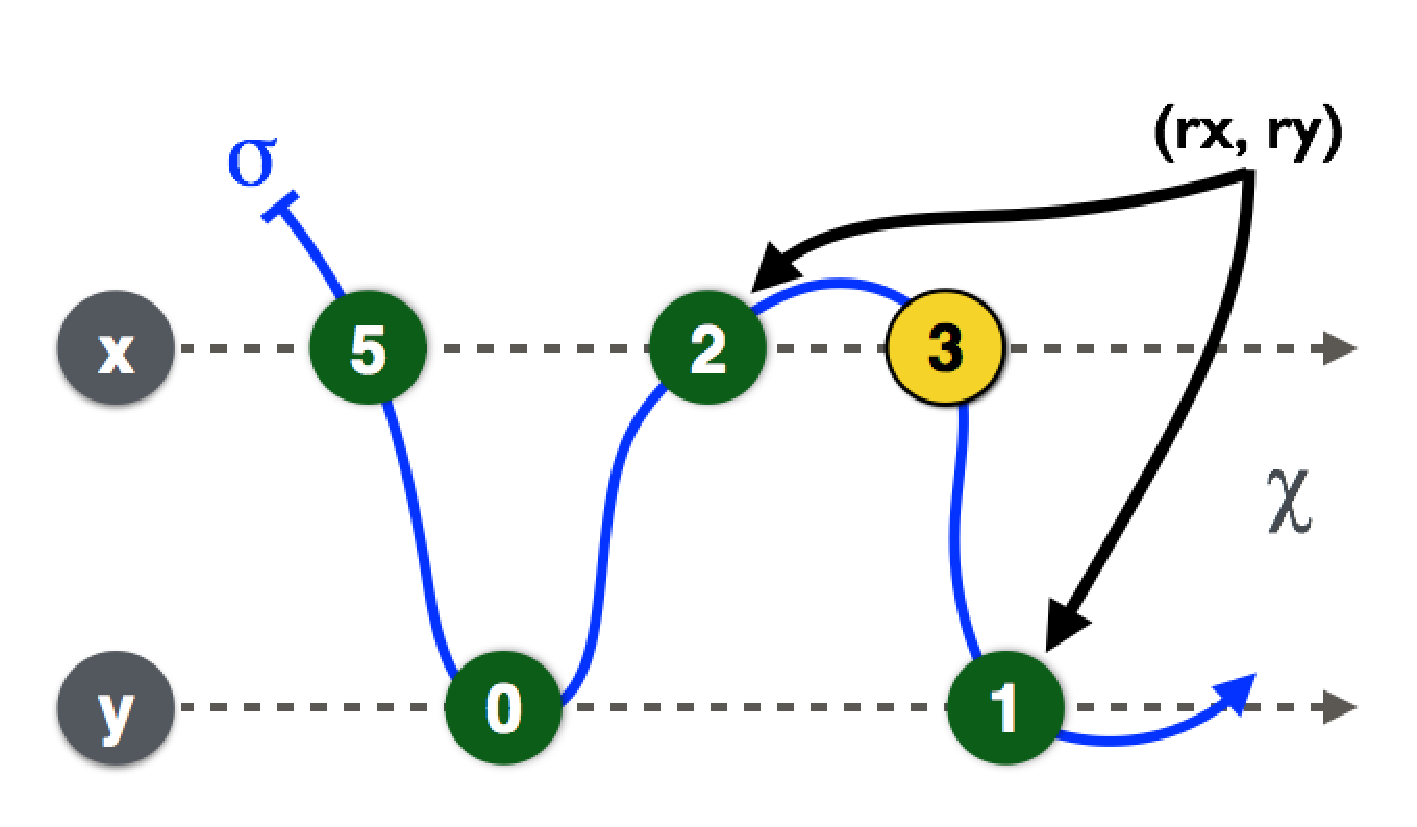
\includegraphics[width=6.1cm]{relink-before3.pdf}
\caption{\label{fig:reorder:before}} % Logical $=$ Real Time order, not a snapshot}
\end{subfigure} \hfill
\begin{subfigure}[t]{0.49\textwidth}
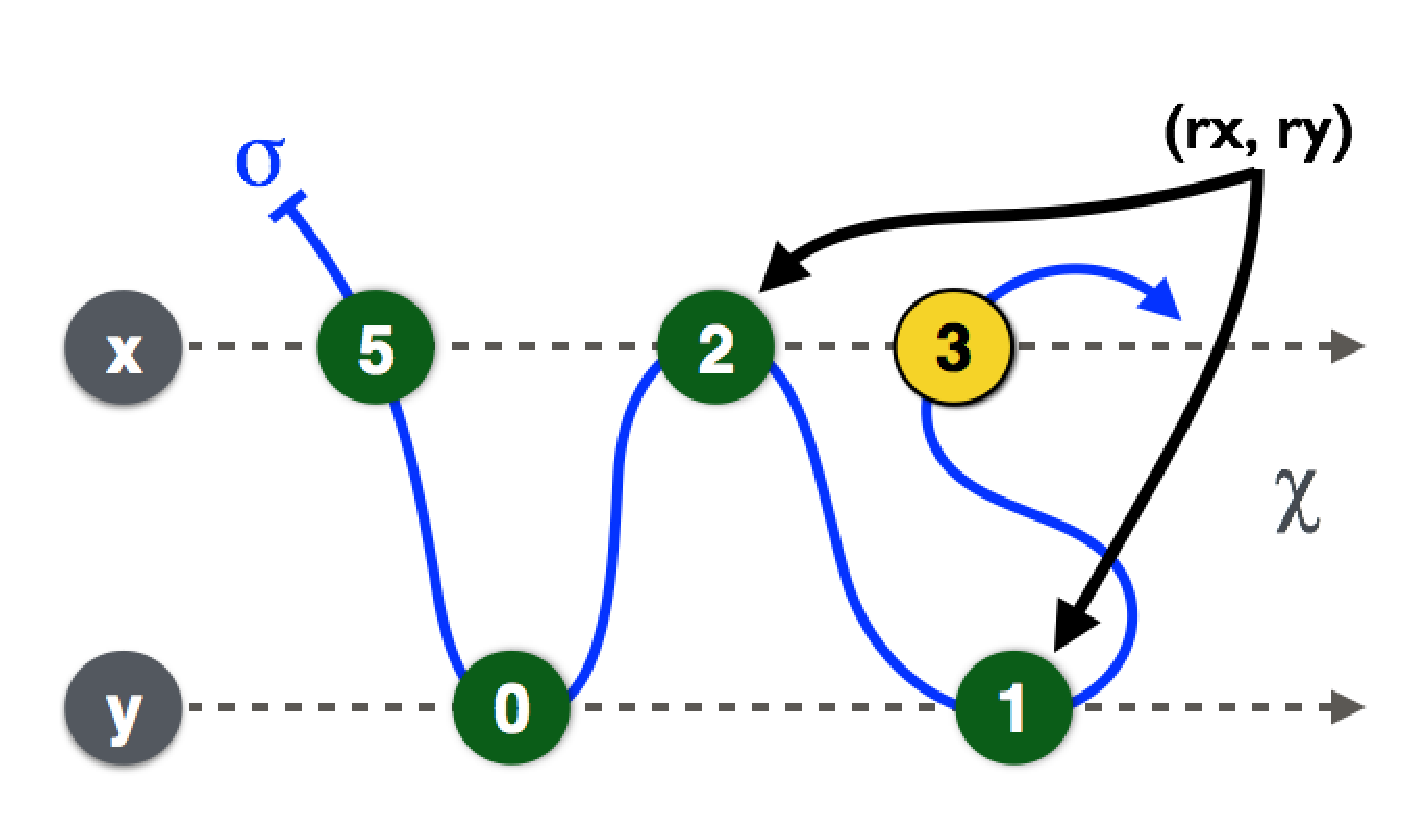
\includegraphics[width=6.1cm]{relink-after3.pdf}
\caption{\label{fig:reorder:after}} % Logical $\neq$ Real Time order, snapshot OK}
\end{subfigure}%
%
\caption{\label{fig:reorder} Changing the logical ordering (solid line
  $\ordlist$) of write events from (5, 0, 2, 3, 1) in
  (\subref{fig:reorder:before}) to (5, 0, 2, 1, 3) in
  (\subref{fig:reorder:after}), to reconcile with {\tt scan} returning
  the snapshot $\x=2, \y=1$, upon missing the write of $3$. Dashed
  lines $\hist$ represent real-time ordering.}
\end{figure}


Obviously, the high-level pattern of the proof requires tracking the
\emph{logical ordering} of the \jywrite\ and \jyscan\ events, which
differs from their \emph{real-time ordering}. As the logical ordering
is inherently dynamic, depending on properties such as
\jyscan\ missing a \jywrite, we formalize it in Hoare logic, by
keeping it as a list of events in auxiliary state that can be
dynamically reordered as needed. For example, Figure~\ref{fig:reorder}
shows the situation in the execution of \jyscan~that we reviewed
above. We start with the (initializing) writes of $5$ and $0$ already
executed, and our program performs the writes of $2$, $3$ and $1$ in
the real time order shown by the position of the events on the dashed
lines. In Figure~\ref{fig:reorder:before}, the logical order
$\ordlist$ coincides with real-time order, but is unsound for the
snapshot $\x=2, \y=1$ that \jyscan~wants to return. In that case, the
auxiliary code with which we annotate \jyscan, will change the
sequence $\ordlist$ in-place, as shown in
Figure~\ref{fig:reorder:after}.

Our specification and verification challenge then lies in reconciling
the following requirements. First, we have to posit specs that
say that \jywrite\ performs a write, and \jyscan\ performs a scan of
the memory, with the operations executing in a single logical
moment. Second, we need to implement the event reordering discipline
so that a method call only reorders events that overlap with it; the
logical order of the past events should be preserved. This will be
accomplished by introducing yet further structures into the auxiliary
state and code. Finally, the specs must hide the specifics of
the reordering discipline, which should be internal to the snapshot
object. Different snapshot implementations should be free to implement
different reorderings, without changing the method specs.


%Our challenge then lies in reconciling the following two conflicting
%requirements. First, we need to implement the reordering discipline so
%that the subsequent calls to \jywrite~and \jyscan~preserve the
%established logical order of the past events. This will be
%accomplished by introducing yet further structures into the auxiliary
%state and code. Second, we have to engineer Hoare triples for
%\jywrite~and \jyscan~to be \emph{intuitive} and \emph{helpful} to
%clients, but also to \emph{not expose} the specifics of the reordering
%discipline, which is internal to the snapshot object\footnotemark.
%%We discuss these issues next.
%\footnotetext{\ie we want to give the methods {\it principal} specifications}



\section{Formal proof structures}
\label{sc:formal}

\def\histx{\hist_\x}
\def\histy{\hist_\y}
\def\histp{\hist_p}
\def\ordlist{L}
\renewcommand{\tleq}{\mathrel{\leq_\ordlist}}
\renewcommand{\tle}{\mathrel{<_\ordlist}}
\newcommand{\E}{E}
\newcommand{\C}{C}
\newcommand{\sx}{S_\x}
\newcommand{\sy}{S_\y}
\newcommand{\spp}{S_p}
\newcommand{\sss}{S_s}
\newcommand{\wx}{W_\x}
\newcommand{\wy}{W_\y}
\newcommand{\wpp}{W_p}
\newcommand{\admissible}{\mathsf{fine}}

% Names for writer/scanner-states
\def\toff{t_{\mathsf{off}}}
\newcommand{\wInit}{\mathsf{W_{off}}}
\newcommand{\wWrite}{\mathsf{New}}
\newcommand{\wDirty}{\mathsf{NeedsFwd}}
\newcommand{\wClean}{\mathsf{Done}}
\newcommand{\sOn}{\mathsf{S_{on}}}
\newcommand{\sOff}{\mathsf{S_{off}}}

%% \gad{ Leave the beginning of the section as it is up to the auxiliary
%%   state, and then introduce Jayanti's FPs. Then follow to describe how
%%   we are implementing them and how they relate to
%%   Invariants~\ref{inv:forward},~\ref{inv:scanner}
%%   and~\ref{inv:redzone}.}

\paragraph*{Specification.}
%
For the purposes of specification and proof, we record a history of
the snapshot object as a set of entries of the form $t \mapsto (p,
v)$. The entry says that at time $t$ (a natural number), the value $v$
was written into the pointer $p$. Notice that we identify a write
event with a \emph{single} moment in time $t$, in contrast to
linearizability which keeps a time interval. As we shall see,
internally, our proofs record intervals too, but we hide the interval
end-points from the clients. Also, unlike linearizability, we do not
need to (though we could) keep track of scan events. Scans do not
modify the object state in ways observable by clients, and may thus be
omitted from specifications. These two points illustrate the
improvement in information hiding over linearizability that we
mentioned in Section~\ref{sc:intro}.

%Unlike in the linearizability proof of the snapshot structure, we keep
%only write events in the history. The scan events do not modify the
%abstract state of the structure observable by clients, and can thus be
%omitted to simplify the reasoning process.

The auxiliary variables $\histS$ and $\histO$, which are local to the
specification, record the \emph{finished} write events of each
procedure, and of the interfering environment, respectively.  We also
have a local variable $\histJ$, which records the set of write events
\emph{in progress}. When a call to {\tt write} is initiated, an
auxiliary code places a write entry into $\histJ$; when a call
finishes, the entry is moved from $\histJ$ to $\histS$.
%
%When one thread changes its own $\histS$, this immediately changes
%every other thread's $\histO$---a discipline provided automatically by
%FCSL. 
%
We name by $\hist$ the union $\histS \hunion \histO \hunion \histJ$,
which is the history of the overall snapshot data structure. This is a
\emph{disjoint union}, enforcing that $\histS$, $\histO$ and $\histJ$
do not contain common timestamps.

The timestamps in $\hist$ determine the \emph{real-time} ordering of
write events. We record the \emph{logical} ordering in another
auxiliary variable $\ordlist$, whose type is list (i.e., mathematical
sequence). This list stores the permutation of timestamps from
$\hist$, and we write $t_1 \tleq t_2$ if $t_1$ appears before $t_2$ in
$\ordlist$. The list $\ordlist$ is the ``linking-in-time'' for the
snapshot algorithm, and can be dynamically modified by the threads.
%
%In this sense, $\ordlist$ is the linkage in time for the snapshot
%algorithm, and it will be dynamically modified. 
%
The order $\tleq$ is total (i.e., a chain), but as $\tleq$ is dynamic,
we introduce further notation, and name by $\jleq{\ordlist}$ a \emph{partial
  suborder} of $\tleq$ that is \emph{stable}, i.e., it can only grow
over time to add new relations, but cannot change the old ones. 
%
For example, in Figure~\ref{fig:reorder}, the initial value of $\tleq$ is
(in lattice notation) $5{-}0{-}2{-}3{-}1$, which changes to $5{-}0{-}2{-}1{-}3$. Stable
order $\jleq{\ordlist}$ is the lattice
$5{-}0{-}2{<}\!\!\!\begin{array}[c]{c}1\\ 3\end{array}\!\!\!$: $1$ and $3$ are unrelated.

We will formally define $\jleq{\ordlist}$ later, but we can already use it to
give Hoare triples for {\tt write} and {\tt scan}. In fact, it will be
important for client reasoning (Section~\ref{sec:clients}) to keep the
definition of $\jleq{\ordlist}$ \emph{hidden}, so that different snapshot
algorithms can provide different definitions, without influencing the
clients.
%
% The following version saves a little more space
\begin{figure}
%
\centering
\[
\begin{array}{l}
\mathtt{write}\ (p : \mathtt{ptr}, n : \mathtt{int}) : 
\!\!\!\begin{array}[t]{l}
\{\hists = \hempty \wedge h \subseteq \histO
           \wedge \omega \subseteq {\jleq}\}\\[3pt]
\{\exists t\ldot\, \hists = t \mapsto (p, n) \wedge h \subseteq \histO \wedge
  \omega \subseteq {\jleq}\,{\wedge}\, h \subseteq H^{\hbox{}\sqsubsetneq_\ordlist t}\}
\end{array}\\
%
\mathtt{scan} : 
\!\!\!\begin{array}[t]{l}
\{\hists = \hempty \wedge\, h \subseteq \histO \wedge\,
          \omega \subseteq {\jleq}\}\\[3pt]
          \{\hists = \hempty \wedge\, h \subseteq \histO \wedge\,
            \omega \subseteq {\jleq} \wedge\, \exists\, t\ldot\, %
             h \subseteq H^{\hbox{}\sqsubseteq_\ordlist t} \wedge\,
             \mathsf{chain}\ H^{\hbox{}\sqsubseteq_\ordlist t} \wedge\,
             r = \mathsf{eval}\ {H^{\hbox{}\sqsubseteq_\ordlist t}}\}
       \end{array}
\end{array}
\]
\caption{\label{fig:specs} Specification of {\tt write} and {\tt scan}
  methods.}
\end{figure}

%% \begin{equation}
%% \begin{array}{l}
%% \mathtt{write}\ (p : \mathtt{ptr}, n : \mathtt{int}) : 
%% \!\!\!\begin{array}[t]{l}
%% \{\hists = \hempty \wedge h \subseteq \histO
%%            \wedge \omega \subseteq {\jleq{\ordlist}}\}\\[3pt]
%% \{\exists t\ldot\, \hists = t \mapsto (p, n) \wedge h \subseteq \histO \wedge
%%   \omega \subseteq {\jleq{\ordlist}}\,{\wedge}\, h \subseteq H^{\hbox{}\sqsubsetneq_\ordlist t}\}
%% \end{array}\\
%% %
%% \mathtt{scan} : 
%% \!\!\!\begin{array}[t]{l}
%% \{\hists = \hempty \wedge\, h \subseteq \histO \wedge\,
%%           \omega \subseteq {\jleq{\ordlist}}\}\\[3pt]
%% \{\hists = \hempty \wedge\, h \subseteq \histO \wedge\, \omega \subseteq {\jleq{\ordlist}} \wedge\, \exists\, t\ldot\, %
%%            h \subseteq H^{\hbox{}\sqsubseteq_\ordlist t} \wedge\,
%%            \mathsf{chain}\ H^{\hbox{}\sqsubseteq_\ordlist t} \wedge\, r = \mathsf{eval}\ {H^{\hbox{}\sqsubseteq_\ordlist t}}\}
%% \end{array}
%% \end{array}
%% \label{eq:specs}
%% \end{equation}
%
Figure~\ref{fig:specs} presents our specifications for {\tt write} and
{\tt scan}. These are partial correctness Hoare triples, describing
how the program changes the state from the precondition (first braces)
to the postcondition (second braces), possibly influencing the return
result $r$. %, in the postcondition of {\tt scan}.
%
The expression $H^{\hbox{}\jleq{\ordlist} t}$ selects the entries in the history
$H$ \emph{up to and including} the timestamp $t$, according to the
ordering $\jleq{\ordlist}$. Likewise, $H^{\hbox{}\sqsubsetneq_\ordlist t}$ is
defined to exclude $t$.
%
We describe the specifications next, before commenting on their
relationship to linearizability.

The specification for {\tt write} says the following. We start with
the empty self history indicating that the procedure did not yet make
any writes. We use the variable $h$ to name an arbitrary subset of the
initial value of $\histO$ (hence, of \emph{completed} write events of
\emph{all other threads}), and the variable $\omega$ for a subset of
the initial ordering $\jleq{\ordlist}$. The postcondition says that when {\tt
  write} terminates, one write event $t \mapsto (p, v)$ has finished,
and is hence placed into $\histS$.  $\histO$ and $\jleq{\ordlist}$ may have
changed from the previous values, due to interference, but they still
include $h$ and $\omega$ as subsets. That is, $\histO$ could only
grow, because other threads could create new write events, and
similarly for $\jleq{\ordlist}$. Lastly, the conjunct $h \subseteq
H^{\hbox{}\sqsubsetneq_\ordlist t}$ says that the write events that
have been completed before the call to {\tt write} (and are hence
stored in $h$) will be \emph{ordered before} the event $t$ in $\jleq{\ordlist}$,
no matter how $L$ is permuted by interfering threads. In other words,
we cannot logically reorder past events, which is a basic soundness
requirement. But notice how stating it requires that $\histO$ is in
scope, thus directly relating {\tt write} to the interfering threads.

The specification for {\tt scan} starts with the same precondition. In
the postcondition, it says that $\histS$ is empty, because {\tt scan}
itself does not create write events. However, by the time {\tt scan}
returns the pair $r$ as a snapshot, we know that there exists a
timestamp $t$ in the collective history $H$ at which the snapshot
\emph{appears} to be taken. First, the conjunct $h \subseteq
H^{\hbox{}\jleq{\ordlist} t}$ indicates that the snapshot is taken \emph{after}
the call to {\tt scan}, because the finished events stored in $h$ are
ordered before (or at best, at) timestamp $t$.
%
%% Second, the set $H^{\hbox{}\sqsubseteq_\ordlist t}$ is
%% a subchain in $\sqsubseteq_\ordlist$ (technically, all its entries are
%% ordered in $\sqsubseteq_\ordlist$).
%
%
Second, the timestamps from $H^{\hbox{}\jleq{\ordlist} t}$ form a sub-chain in
$\jleq{\ordlist}$,  % (\ie, $\forall\, a,b \in H^{\hbox{}\sqsubseteq_\ordlist
%  t}\ldot\ a \sqsubseteq_{\ordlist} b \vee b \sqsubseteq_{\ordlist}
%a$.
%
encoding how the writes progressed logically in time up to the
snapshot moment $t$. Moreover, since $\jleq{\ordlist}$ is stable, this view
of the time will not change in the future to invalidate the result $r$
as a snapshot. Finally, if the chain of writes is evaluated in the
order given by $\jleq{\ordlist}$, it produces $r$.

%\gad{Actually, proving that chain is stable entails proving something
%  stronger: that the sub-chain $H^{\hbox{}\sqsubseteq_\ordlist t}$ is
%  ``maximal'' or complete i.e. that no more entries are going to be
%  added to that sub-history. This is (will be) proven by the fact that
%  in the atomic moment after we have executed re-link,
%  $H^{\hbox{}\sqsubseteq_\ordlist t}$ defines a green prefix from the
%  very beginning up to the timestamp t, and such prefixes are stable.}

Notice how these specifications directly capture what linearizability
would have given us: in both procedures we get a time moment $t$ at
which the procedure executed \emph{logically instantaneously}, as part
of a larger \emph{sequence} $H$. Additionally, {\tt write} performed a
write event at $t$, and {\tt scan} returned a snapshot consistent with
scanning at $t$. In the case of linearizability, the last property
requires showing a simulation between the concurrent implementations
of {\tt write} and {\tt scan}, and some sequential equivalents. If we
then want to verify Hoare triples of clients, we need to establish
Hoare triples for the sequential equivalents. In our method, the
process is streamlined by immediately giving Hoare triples for the
concurrent implementations, avoiding intermediary sequential
equivalents and simulation proofs.

\paragraph*{Internal auxiliary state.} 
The proofs of {\tt write} and {\tt scan} require further auxiliary
state, which does not feature in the specifications, and is hence
hidden from clients.

First, we track the point of execution in which {\tt write} and {\tt
  scan} are, but instead of line numbers in the code, we use
datatypes, to encode extra information in the constructors.
%
For example, the scanner's state is a triple $(\sss, \sx,
\sy)$. $\sss$ is drawn from $\{ \sOn, \sOff\, t\}$. If $\sOn$, then
the scanner is in lines 8--10 in Figure~\ref{fig:jayanti-snapshot}. If
$\sOff\ t$, the the scanner reached line 11 at time $t$, and is now in
11--15.  $\sx$ is a boolean, set when the scanner clears $\fx$ in
line~9, and reset upon scanner's termination (dually for $\sy$ and
$\fy$).
%
Writers' state for $x$ is tracked by the auxiliary $\wx$ (dually,
$\wy$). These are drawn from $\{\wInit, \wWrite\ t, \wDirty\ t,
\wClean\ t\}$, where $t$ marks the beginning of the write. If
$\wInit$, then no write is in progress. If $\wWrite\ t$, then the
writer is in line~2. If $\wDirty\ t$, then $b$ has been set in line~3,
triggering forwarding. If $\wClean\ t$, the writer is free to exit.

Second, like in linearizability, we record the ending times of
events. We use the auxiliary variable $\E$, which is a function
mapping a timestamp $t$ of a \emph{finished} write event from $\hist$,
to a timestamp identifying the event's \emph{ending time}. Events
$t_1$ and $t_2$ which are non-overlapping (i.e., $E(t_1) < t_2$ or
$E(t_2) < t_1$), will never be reordered, thus {\tt write} and {\tt
  scan} cannot modify the past history.

%Formally, the
%following is an invariant of the algorithm.
%\vspace{-2mm}

\begin{proposition}\label{inv:overlap}%
%The logical order $\tle$ preserves the real time order of {\it
%  non-overlapping} past write events. Formally, 
$\forall t_1 \in \dom{E}, t_2 \in \dom{\hist}$, if $E(t_1) < t_2$
  then $t_1 \tle t_2$.
\end{proposition}

Third, we track the rearrangement status of write events wrt.~an
ongoing \emph{active} scan, by \emph{colors}. A scan is \emph{active}
if it has cleared the forwarding pointers in line~9, and is ready to
read $x$ and $y$. The auxiliary variable $\C$ is a function mapping
each timestamp in $\hist$ to a color, as follows.
%
%% It is always relative to the ongoing scan, or the last finished one,
%% if no scans are active.
%
\begin{itemize}
\item {\sf Green} timestamps identify events whose position in the
  logical order is fixed in the following sense: if $\C(t_1) =
  \mathsf{green}$ and $t_1 \tle t_2$, then $t_1 <_{\ordlist'} t_2$ for
  every $\ordlist'$ to which $\ordlist$ may step by auxiliary code
  execution (Section~\ref{sc:implementation}). For example, since we
  only reorder overlapping events, and only the scanner reorders
  events, every event that finished before the active scan started
  will be green. Also, a green timestamp never changes the color.
\item {\sf Yellow} timestamps identify events whose order is not fixed
  yet (i.e., they are not linearized), but which \emph{may} be
  manipulated by the ongoing active scan, as follows.  The scan can
  \emph{push} a yellow timestamp in logical time, \emph{past} another
  green or yellow timestamp, but not past a red one. \emph{This is the
    only way the logical ordering can be modified.}

\item {\sf Red} timestamps identify events whose order is not fixed
  yet, but which will \emph{not} be manipulated by the active scan,
  and are left for the next one.
%
%% They
%% will be put after the green ones.
\end{itemize}
%

There is a number of invariants that relate colors and timestamps. For
brevity, we only list the most important ones, and defer to the Coq
code for the others~\cite{CoqFiles}. In the sequel, we use
$\histp$ to denote the set of writes into the pointer $p$ that appear
in the history $\hist$.

% Color invariant
\begin{proposition}[Color Invariant]\label{inv:color}%
The colors of $\histp$ are described by the regular expression $\GYR$:
there is a non-empty prefix of green timestamps, followed by \emph{at
  most} one yellow, and arbitrary number of reds.
\end{proposition}

This proposition identifies, by the yellow color, the write event for
$p$ that is the unique candidate for reordering by the ongoing active
scan. Moreover, all the writes into $p$ prior to the yellow one, will
have already been painted green (i.e., fixed in time, linearized),
whether they overlapped with the scanner or not.

\begin{comment}
\begin{proposition}[First Forwarding Principle]\label{inv:fwd1}%
If the scanner state is $\sss = \sOff\ \toff, \spp = \TT$, then
$\forall\ t \in \histp\ldot\ t \leq \E(t)< \toff \implies \C(t)=
\mathsf{green}$.
\end{proposition}
%
The above is our mathematical formulation approximating the
equally-named, but only informally stated property of
Jayanti~\cite{Jayanti:STOC05}, which says that if {\tt scan} misses
the value of a concurrent write in line~10 of
Figure~\ref{fig:jayanti-snapshot}, but the write finishes before the
scanner goes through line~11 (the scan's linearization point), then
the scanner will catch the value in the forwarding pointer in
line~12. In our setting, this is captured by saying that a write event
that finished before $\toff$, is green. The write event may have been
yellow in the past, but the act of forwarding will paint it green. We
will see in Section~\ref{sc:implementation} that auxiliary code for
forwarding will do just that.

%It is easy to see how this proposition corresponds to Jayanti's First
%Forwarding Priciple: in our seeting a write event which is visible,
%ergo never going to be missed is {\sf green}. Then the Proposition
%above says that any write event that finished strictly before $\toff$
%will be green. This means that in the case that a write event was
%committed to memory after the scanner read in line 10-- in which case
%it was originally painted {\sf yellow} ---it must have been forwarded,
%as forwarding paints entries from yellow to green. As for the Second
%Forwarding Principle, we capture it through the two following
%propositions:

Conversely, Jayanti's Second Principle states that any non-$\bot$
value read in line~12 comes from a write event that is concurrent with
the scan. Moreover, any later write to the same pointer will finish
after the linearization point of {\tt scan} in line 11, and hence will
be missed by the scanner. While we do not formally capture exactly
this property, we approximate it with the following two invariants,
which are sufficient.

\end{comment}

%% %% Key Inv for fp
\begin{proposition}[Green/Yellow Forwarded Values]\item\label{inv:readFP} 
If $\sss= \sOff\ \toff$ and $\spp = \TT$ (i.e., scanner is in lines
12--14), and a value $v \neq \bot$ has been forwarded to $p$ (i.e.,
$\mathit{fp} = v$), then the event of writing $v$ into $p$ is in the
history, i.e., exists $t$ such that $t \mapsto (p, v) \in
\histp$. Moreover, $t$ is the last green, or the yellow timestamp in
$\histp$.
%(It can then be
%derived that $t$ must be overlapping with the scan).
\end{proposition}

This proposition restricts the set of events that could have forwarded
a value to the scanner, to only two: the event with the (unique)
yellow timestamp, or the one with the last green timestamp. By
Proposition~\ref{inv:color}, the two timestamps are consecutive in
$\histp$.
 
%% RedZone invariant
\begin{proposition}[Red-Zone Invariant]\label{inv:redzone}%
If $\sss = \sOff\ \toff, \sx = \TT, \sy = \TT$, then $\hist$ satisfies
the $\RZ$ pattern. Moreover, for every $t' \in \mathsf{dom}(H)$:
%
\begin{itemize}
\item $\C(t') = \mathsf{green} \implies t' \leq \toff$
\item $\C(t') = \mathsf{yellow} \implies t' \leq \toff \leq \E (t')$
\item $\C(t') = \mathsf{red} \implies \toff < t'$  
\end{itemize}
\end{proposition}

This proposition restricts the global history $\hist$ (not the
projections $\histp$). First, the red events in $H$ do not mix with
the green and yellow ones. Thus, when a scanner pushes a yellow event
past a green or yellow event, it will not ``jump over'' any reds, thus
keeping the invariant that ordering on reds is not manipulated by the
scan. Second, the proposition relates the colors to the time $\toff$
at which the scanner was turned off (in line~11,
Figure~\ref{fig:jayanti-snapshot}). This moment is important for the
algorithm; e.g., it is the linearization point for {\tt scan} in
Jayanti's proof~\cite{Jayanti:STOC05}.
%
In our proof, the inequalities wrt.~$\toff$ are used to prove that the
events reordered by the scanner \emph{do} overlap, as per
Proposition~\ref{inv:overlap}.

\begin{comment}
Proposition~\ref{inv:readFP} states that any non-$\bot$ value read
from the forwarding pointer $\mathit{fp}$ at line 12 might have been
written to $p$ after the scanner cleared the forwarding pointers, and
and hence, be newer than the values read in line 10. This captures the
essence of the first part of Jayanti's Second forwarding principle.
%
Proposition~\ref{inv:redzone} states that when the scanner is in
between lines 12-15 in Figure~\ref{fig:jayanti-snapshot}, then $\hist$
can be partitioned into a non-empty prefix with yellow and/or green
timestamps, and a reds-only suffix. Moreover, if a new write event $t$
occurs at this point, with $ \toff < t <= \E (t)$, it will be colored
red and hence ignored by the current scanner. This later fact captures
the last part of the second Forwarding Principle. Later on, this
proposition will be crucial into proving that relink does not affect
the order of write events that are meant to missed, by keeping them in
the red suffix, and also that those being reordered are overlapping.

\gad{Explain better? The second part of this invariant might also be
  connected to Jayanti's ``Correctness'' Theorem, Lemma 5 in his
  Appendix. I'm not sure however if I need to express its connection
  here.}
\end{comment}

We can now define the stable logical order $\jleq{\ordlist}$, which relies on
the internal auxiliary state.
%
\begin{definition}[Logical Order]\label{def-jleq}
%\begin{equation*}
$t_1 \jleq{\ordlist} t_2 \eqdef t_1 = t_2 \vee E\,(t_1) < t_2 \vee (t_1 \tle t_2 \wedge \C(t_1) = \mathsf{green})$.
%\end{equation*}
\end{definition}
The proposition $t_1 \jleq{\ordlist} t_2$ is stable (i.e., invariant under
interference), since threads do not change the ending times $E$, the
color of green events, or the order of green events in $\tle$.

%Stability holds because the first two disjuncts do not relate mutable
%values, and the third is stable because green timestamps are not
%reordered nor recolored.
%\gad{Explain stability here}
%
%\gad{Add some comment about Forwarding Principles back in, either here
%  or in Related Work.}
%
%\gad{Add instantiation of the ideal $H^{\hbox{}\sqsubseteq_\ordlist t}
%  $ w.r.t Figures~\ref{fig:weird:exec} and~\ref{fig:reorder}}

%% %
%% \gad{I've changed the definition so that it is closer to its
%%   implementation in the Coq development.}

%% \begin{equation}
%%  t_1 \jleq{\ordlist} t_2  = (t_1 = t_2) \vee (E\,(t_1) < t_2) \vee
%%  (t_1\tle t_2 \wedge \C(t_1) = \mathsf{green}) \label{def-jleq}
%% \end{equation}
%

%% \gad{Introduce Jayanti's forwarding principles and how we implement
%%   them with the colors.  Use this to motivate the invariants in
%%   particular~\ref{inv:wrtP},~\ref{inv:readFP}, and~\ref{inv:redzone},
%%   which are the ones that correspond closely to the forwarding
%%   principles.}

%% \paragraph*{Forwarding Principles}
%% Jayanti introduces two {\it Forwarding
%%   Principles}~\cite{Jayanti:STOC05} that guide the design of his
%% snapshot algorithm and provide an intuition for the correctness of the
%% proof of their linearizability. In essence, the First Principle says
%% that, in Figure~\ref{fig:jayanti-snapshot} if {\tt scan} misses the
%% value of a concurrent write when reads in line~10, if the said writer
%% finishes before line~11 (the scanner method's linearization point),
%% the scanner will catch it by reading the forwarding pointer in
%% line~12.


%% The Second Principle then dually states that any non-$\bot$
%% value read in the latter line comes from a write event's timestimap
%% $t$ concurrent with {\tt scan} and that for any other write event such
%% that $ t < t'$, $t'$ finishes after line 11 in {\tt scan}, and thus
%% has to be missed. We capture the essence of these forwarding
%% principles through a series of propositions and invariants expressed
%% in terms of the auxiliary state described above:

%% %% Formalizing the Forwarding Principles in full detail requires keeping
%% %% track of otherwise unnecesary scanner events in the history. Instead,
%% %% we capture their essence with the following three propositions, based
%% %% on the colors of the write events and the scanner state.

%% %
%% \gad{We actually don't have this statement in the development, but we
%%   can prove it out of the refined colorinvariant color\_inv and
%%   Proposition~\ref{inv:redzone} below. I will add it to the Coq files
%%   to-do list.}

%% It is easy to see how this proposition corresponds to Jayanti's First
%% Forwarding Priciple: in our seeting a write event which is visible,
%% ergo never going to be missed is {\sf green}. Then the Proposition
%% above says that any write event that finished strictly before $\toff$
%% will be green. This means that in the case that a write event was
%% committed to memory after the scanner read in line 10-- in which case
%% it was originally painted {\sf yellow} ---it must have been forwarded,
%% as forwarding paints entries from yellow to green. As for the Second
%% Forwarding Principle, we capture it through the two following
%% propositions:

%% \begin{comment}
%% %%%%%%%%%  
%%  Jayanti's Forwarding Principles: in quote:
%%  '' The first principle ensures that if the scanner misses a Write
%%  at A[i], then it will catch that Write at B[i]. More precisely:

%%   Forwarding Principle 1:Suppose that a Scan operation S misses
%%   aWrite(i, v)operation W because S reads A[i] before W writes in
%%   A[i]. If W completes before S performs Line 7, then W will have
%%   surely informed S of v by writing v in B[i].

%%   The second principle ensures that any non-\bot value that the
%%   scanner may find in B[i]is current. More precisely:

%%   Forwarding Principle 2:Suppose that a Scan opera- tion S reads at
%%   Line 9 a non-\bot value written in B[i]by some Write(i, v)operation
%%   W.Then, (1) W is concurrent with S, and (2) If W′ is any Write(i,
%%   ∗)operation thatis executed after W,then W′ completes only after S
%%   performs Line 7. (...)''
%% %%%%%%%%
%% \end{comment}

%% %% Key Inv for P
%% \begin{proposition}[Green/Yellow Writes]\item\label{inv:wrtP}%
%% For each of $\histx, \histy$, if the scanner state is $\sss= \sOn,
%% \spp = \TT$, i.e., it is in lines 9--11 in
%% Figure~\ref{fig:jayanti-snapshot}, and $ \mathit{p} = v$ in the
%% physical state, then this is recorded by $\histp$: $\exists t\ldot t
%% \mapsto (p, v) \in \histp$. Moreover, $t$ will be considered by the
%% scanner, i.e., $t$ is the last green or the yellow timestamp in
%% $\histp$.
%% \end{proposition}

%% \gad{I'm not sure Proposition~\ref{inv:wrtP} is helpful here}
  

%% \gad{We might need to explain the new part of the red-zone invariant
%%   i.e. the one that explains the relation between the timestamps of
%%   the writes and $t_{\mathsf{off}}$. This is important for
%%   establishing that re-link only changes the order of overlapping
%%   events.}

%% In order to prove the correctness of these specs, we introduce the
%% invariants imposed on our axiliary state, as well as the
%% implementation in FCSL of the algorithm, decorated with auxiliary
%% code:

%% \paragraph*{Invariants}%
%% The following are (selected) properties relevant to the proof of the
%% specs, that the state (real and auxiliary) of the snapshot algorithm
%% satisfies throughout execution.
%% \an{Some are mostly obvious
%%   book-keeping properties, but some are essential. We should present
%%   only the important ones.}

%% % Self/other histories record finish
%% writes.  \item\label{inv:gapless} $\hist$ is gapless, i.e.,
%% contains all the timestamps between $0$ and the maximal
%% one. Moreover, each timestamp is associated with either the pointer
%% $x$ or the pointer $y$; if we denote by $\histx$ and $\histy$ the
%% entries in $\hist$ writing into $x$ and $y$ respectively, then
%% $\hist = \histx \hunion \histy$. \an{removable?} \gad{yes}

%% % Self/other histories record finish
%% writes.  \item\label{inv:finished} $\histS$ and $\histO$ record
%% finished writes: $\dom{E} = \dom{\histS \hunion
%% \histO}$. \an{removable?} \gad{yes}

% Color invariant
%% \item\label{inv:color} The colors of the timestamps in each of
%%   $\histx$ and $\histy$ can be described by the regular expression
%%   $\GYR$: They have a non-empty prefix consisting of green timestamps,
%%   followed by \emph{at most} one yellow timestamp, and zero or more
%%   red timestamps in the tail.
%%   %
%%   %% Importantly, there is always a (green)
%%   %%  entry describing the initial write into each $x$ and $y$.
%
%  i.e. the coloring of each of the pointer-view histories satisfies
%  the pattern: many (at least one) green, at most one yellow, zero or
%  more red. \gad{Will I need the refinements?}. This pattern entails
%  that there is an initial value in each of $\histx$ and $\histy$ and,
%  moreover, that initial write is {\bf green}. One of those initial
%  timestamps will be $0$, i.e. $C(0)= green$. In addition, each
%  pointer-view history is sorted in real time -- naturally sorted--
%  and its elements don't overlap.

%% Non-Overlapping are sorted
%% \item\label{inv:overlap} The ending real time of a finished event
%%   appears after the initial real time: $\forall\, t \in
%%   \dom{E}\ldot\ t \leq E(t)$. \an{removable?}  Moreover, events that
%%   do not overlap in real time are ordered in logical time: $\forall
%%   t_1 \in \dom{E}, t_2 \in \dom{\hist}$, if $E(t_1) < t_2$ then $t_1
%%   \tle t_2$.
  
%% %% Last keys
%% \item\label{inv:lastkey} The entry of the last timestamp in $\histx$
%%   contains the physical value of $\x$: $\x = \histx (\mathsf{last}\,
%%   \histx)$. Similarly for $y$. \an{removable?} \gad{yes}.

%% %% Key Inv for fp
%% \item\label{inv:forward} If the scanner has cleared $\mathit{fx}$
%%   ($\sx = \TT$) but a non-$\bot$ value $v$ has been forwarded since
%%   ($\mathit{fx} = v$), then this is recorded by $\histx$:
%%   $\exists t\ldot t \mapsto (x, v) \in \histx$. Moreover, $t$ will be
%%   considered by the scanner, i.e., $t$ is the last green or the yellow
%%   timestamp in $\histx$. Dually for $\y$.

%% %  For each $\mathtt{p} \in \{\mathtt{x},\mathtt{y}\}$, if $(S_p \wedge
%% %  \mathtt{f\_of\ p}= v)$ then exists $t_p$ such that $t_p \hpts (p,v)
%% %  \in \hist$ and $t_p$ is the last green or yellow timestamp of
%% %  $\hist_{\mathtt{p}}$ i.e. $t_x = \mathsf{last\_green}\ \histx \vee
%% %  t_p = \mathsf{yellow\_ts}\ \hist_{\mathtt{p}}$. This property
%% %  entails that after the scanner has cleared the forwarding pointers,
%% %  if some new value has been forwarded, its timestamp is the last
%% %  green or the yellow of the pointer's view-history.

%% %% Key Inv for p
%% \item\label{inv:scanner} If the scanner has cleared $\mathit{fx}$
%%   ($\sx = \TT$), but still has not turned off $\s$ (i.e., it is in
%%   lines 9-11 in Figure~\ref{fig:jayanti-snapshot}), and $\x = v$ in
%%   physical state, then this is recorded by $\histx$:
%%   $\exists t\ldot t \mapsto (x, v) \in \histx$. Moreover, $t$ will be
%%   considered by the scanner, i.e., $t$ is the last green or the yellow
%%   timestamp in $\histx$. Dually for $\y$.

%  For each $\mathtt{p} \in \{\mathtt{x},\mathtt{y}\}$, if $(S_p
%  \wedge \mathtt{S})$ then exists $t_p$ such that $t_p \hpts (p,v) \in
%  \hist$ and $t_p$ is, again, the last green or yellow timestamp of
%  $\hist_{\mathtt{p}}$ i.e. $t_x = \mathsf{last\_green}\ \histx \vee
%  t_p = \mathsf{yellow\_ts}\ \hist_{\mathtt{p}}$. This property
%  entails that after the in the scanner has cleared the forwarding
%  pointers and before it unsets the scanner bit {\tt S}, the current
%  value of the pointer was committed by the last green or the yellow
%  timestamp of the pointer's view-history.

%% %% RedZone invariant
%% \item\label{inv:redzone} 
%% %
%% If $\s = \FF, \sx = \TT, \sy = \TT$, i.e., the scanner is in lines
%% 12-15 in Figure~\ref{fig:jayanti-snapshot}, then $\hist$ satisfies the
%% $\RZ$ pattern. In other words, if a new write events occur at this
%% point, it will be colored red, and hence ignored by the scanner.

%If $\wstate{S} = (\FF,\TT,\TT)$ then $\hist$ satisfies the $\RZ$
%coloring pattern: if there is a red timestamp in $\hist$, then then
%the {\sf first} red timestamp partitions $\hist$ so that everything
%before it is yellow or green and everything starting from it is red.
  
%\end{enumerate}
%\gad{to do: I'm not sure how deep I should get into the invariants?
%  Won't know for sure until I finish with the proof sketch. We might
%  cut down on them later.}

%\gad{Also: I'm thinking of pushing the invariants down together with
%  the proof sketch, or even fork them together as a separate section
%  sketching the ``correctness'' of our approach}

%% Jayanti's Forwarding Principles are guidelines for the design of the
%% algorithm and also the definition of the Linearization
%% Points. Instead, our implementation of them, as provided by
%% Propositions~\ref{inv:fwd1},~\ref{inv:readFP}, and~\ref{inv:redzone},
%% are formally implemented as invariants of the auxiliary state of the
%% data structure--- or {\it concurrent resource} in FCSL's jargon. In
%% the following we present the atomic auxiliary code operations that
%% implement {\tt write} and {\tt scan} in FCSL. These will be required
%% to satisfy the propositions introduced above, amongst other
%% requirements.

%% \an{Should we make the point that the auxiliary code constructivelly
%%   builds and evolves the various total and partial orderings that are
%%   abstracted by the specifications. It is thus an inherent component
%%   of the proof, in the same way that in type theory, existentials
%%   require a witness. There's probably no space to bring type theory
%%   into the mix.}



\begin{figure}[t]
%
\centering
\begin{tabular}{c@{\hfill}c}
%
\begin{minipage}[t]{.5\textwidth}
\[
\begin{array}{ll}
\num{1}~ & ~~ \esc{write}\ (p,\, v)\ \{\\ 
\num{2}~ & ~~~~~ \lat\,\actwrite{p}{v}; \aux{register}(p,v)\rat;\\
\num{3}~ & ~~~~~ \lat\, b \tbnd \act{read}(S);\ \aux{check}(p,b) \rat;\\
\num{4}~ & ~~~~~ \kw{if}\ b\\
\num{5}~ & ~~~~~ \kw{then}\ \lat\,%
                           \actwrite{\aleksfwdp{p}}{v};\ \aux{forward}(p)\rat; \\
\num{5'}~           & ~~~~ \lat\,\aux{finalize}(p)\rat\}
\end{array}
\]
\end{minipage}
%
&
%
\begin{minipage}[t]{.5\textwidth}
\[
\begin{array}{rl}
\num{6}~  & \esc{scan} () : ( A \times A )~ \{ \\ 
\num{7}~  & ~~~ \lat\,\actwrite{\s}{\esc{true}};\ \aux{set}(\esc{true}) \rat;\\  
\num{8}~  & ~~~ \lat\,\actwrite{\fx}{\bot};\ \aux{clear}(\x)\rat;\\
\num{9}~  & ~~~ \lat\,\actwrite{\fy}{\bot};\ \aux{clear}(\y)\rat;\\
\num{10}~ & ~~~ \var{vx} \tbnd \lat \act{read}(\x) \rat ; \\
\num{11}~ & ~~~ \var{vy} \tbnd \lat \act{read}(\y) \rat;  \\
\num{12}~ & ~~~ \lat\,\actwrite{\s}{\esc{false}};\ \aux{set}(\esc{false})\rat;\\
\num{13}~ & ~~~ \var{ox} \tbnd \lat \act{read}(\fx) \rat;\\
\num{14}~ & ~~~ \var{oy} \tbnd \lat \act{read}(\fy) \rat;\\
\num{15}~ & ~~~ \var{rx} \tbnd \kw{if}\ (\var{ox} \neq\bot)\
                \kw{then}\ \var{ox}\ \kw{else}\ \var{vx};\\
\num{16}~ & ~~~ \var{ry} \tbnd \kw{if}\ (\var{oy} \neq\bot)\
                \kw{then}\ \var{oy}\ \kw{else}\ \var{vy};\\
\num{17~} & ~~~ \lat\,\aux{relink}(\var{rx}, \var{ry});\
                \kw{return}\ (\var{rx}, \var{ry})\,\rat\}
\end{array}
\]
\end{minipage}
%
\end{tabular}
%
\caption{Snapshot procedures annotated with auxiliary code.}
\label{fig:fcsl-snapshot}
\end{figure}




\section{Auxiliary code implementation}
\label{sc:implementation}

%\paragraph*{Implementation}%

Figure~\ref{fig:fcsl-snapshot} annotates Jayanti's procedures with
auxiliary code (typed in \emph{italic}), with $\langle\mbox{angle
braces}\rangle$ denoting that the enclosed real and auxiliary code
execute \emph{simultaneously} (\ie, atomically). The auxiliary code
builds the histories, evolves the sequence $\ordlist$, and updates the
color of various write events, while respecting the invariants from
Section~\ref{sc:formal}. Thus, it is the \emph{constructive} component
of our proofs. Each atomic command in Figure~\ref{fig:fcsl-snapshot}
represents one \emph{transition} of the STS $C$ from
Figure~\ref{fig:specs}.

%
%As customary, auxiliary code is \emph{erasable} at run time; it does
%not mutate the real state.
%
%% We name auxiliary code as one would name procedure calls, and proceed
%% to describe these procedures.
%

The auxiliary code is divided into several procedures, all of which
are sequences of reads followed by updates to auxiliary variables. We
present them as Hoare triples in Figure~\ref{fig:auxcode}, with the
unmentioned state considered unchanged. The bracketed variables
preceding the triples (\eg, $[t, v]$) are logical variables used to
show how the pre-state value of some auxiliary changes in the
post-state. To symbolize that these triples \emph{define} an atomic
command, rather than merely stating the command's properties, we
enclose the pre- and postcondition in angle brackets $\langle
- \rangle$.

%Following are the characteristic cases.

% %%\usetikzlibrary{arrows,shapes,automata, positioning}
\usetikzlibrary{arrows,shapes,automata,positioning}

%% \begin{figure}[ht]
%% \begin{subfigure}[t]{.4\textwidth}
%% \centering
%% \small
%% \begin{tikzpicture}[->,>=stealth',shorten >=1pt,auto,node distance=3cm,
%%                     thick,initial text={},initial above]
%%   \tikzstyle{every state}=[fill=white,draw,ellipse,text=black]
%%   \node[initial,state] (A)                    {$\mathsf{Init}$};
%%   \node[state]         (B) [below right of=A] {$\mathsf{Written\ t}$};
%%   \node[state]         (D) [below left of=A] {$\mathsf{Clean\ t}$};
%%   \node[state]         (C) [below left of=B] {$\mathsf{Dirty\ t}$};
 
%%   \path (A) edge [bend left]  node {$\act{register}(p,v)$} (B)
%%         (B) edge [bend left]  node {$\act{check}(p,true)$} (C)
%%             edge              node {$\act{check}(p,false)$} (D)
%%         (C) edge [bend left]  node {$\act{forward}(p)$}(D)
%%         (D) edge [bend left]  node {$\act{exit}()$} (A);
%% \end{tikzpicture}
%% \caption{\label{fig:sts:writer} Write STS on $\wstate{p}$}
%% \end{subfigure}%
%% \begin{subfigure}[t]{.6\textwidth}
%% \centering
%% \small
%% \begin{tikzpicture}[->,>=stealth',shorten >=1pt,auto,node distance=2.2cm,
%%                     thick,initial text={},]
%%   \tikzstyle{every state}=[fill=white,draw,ellipse,text=black]
%%   \node[initial,state] (A)                     {$(\FF,\FF,\FF)$};
%%   \node[state]         (B)  [above right of=A] {$(\TT,\FF,\FF)$};
%%   \node[state]         (C1) [above right of=B] {$(\TT,\TT,\FF)$};
%%   \node[state]         (C2) [below right of=B] {$(\TT,\FF,\TT)$};
%%   \node[state]         (D)  [right=2.5 cm of B]  {$(\TT,\TT,\TT)$};
%%   \node[state]         (E)  [below right=0.5cm and 0.cm of C2]
%%                               {$(\FF,\TT,\TT)$};
%%   \path (A)  edge [bend left]   node {$\act{set}(\TT)$} (B)
%%         (B)  edge [bend left]   node {$\act{clear}(\mathtt{x})$} (C1)
%%              edge [bend right]  node {$\act{clear}(\mathtt{y})$} (C2)
%%         (C1) edge [bend left]   node {$\act{clear}(\mathtt{y})$} (D)
%%         (C2) edge [bend right]  node {$\act{clear}(\mathtt{x})$} (D)
%%         (D)  edge [bend left]   node {$\act{set}(\FF)$} (E)
%%         (E)  edge [bend left]   node {$\act{relink}(rx,ry)$} (A);
%% \end{tikzpicture}
%% \caption{\label{fig:sts:scanner} Scan STS on $\wstate{S}$}
%% \end{subfigure}
%%  \caption{\label{fig:sts} The State Transition System described by auxiliary code}
%% \end{figure}

% I don't need the scanner protocol at all
%\begin{figure}

\begin{figure}
\small
\begin{tikzpicture}[->,>=stealth',shorten >=1pt,auto,node distance=3cm,
                    thick,initial text={},initial above]
  \tikzstyle{every state}=[fill=white,draw,ellipse,text=black]
  \node[initial,state] (A)                    {$\wInit$};
  \node[state]         (B) [below right of=A] {$\wWrite\ t$};
  \node[state]         (D) [below left of=A] {$\wClean\ t$};
  \node[state]         (C) [below left of=B] {$\wDirty\ t$};
 
  \path (A) edge [bend left]  node {$\act{register}(p,v)$} (B)
        (B) edge [bend left]  node {$\act{checkS}(p,true)$} (C)
            edge              node {$\act{checkS}(p,false)$} (D)
        (C) edge [bend left]  node {$\act{forward}(p)$}(D)
        (D) edge [bend left]  node {$\act{finalize}()$} (A);
\end{tikzpicture}
\caption{\label{fig:sts-writer} \jywrite's auxiliary code implements a STS on writer states $\wpp$.}
\end{figure}

\begin{figure}
\small
\begin{tikzpicture}[->,>=stealth',shorten >=1pt,auto,node distance=2cm,
                    thick,initial text={},]
  \tikzstyle{every state}=[fill=white,draw,ellipse,text=black]

  \node[] (I) [] {};
  \node[] (X) [above=1.5 cm of I] {}; 
  \node[state]         (B)  [left=0.5 cm of X]  {$(\sOn,\FF,\FF)$};
  \node[state]         (C)  [right=0.5 cm of X] {$(\sOn,\TT,\FF)$};
  \node[initial,state] (A)  [left= 1.5 cm of I] {$(\sOff\ \_,\FF,\FF)$};
  \node[state]         (D)  [right= 1.5 cm of I] {$(\sOn,\TT,\TT)$};
  \node[state]         (E)  [below=1 cm of I] {$(\sOff\ t,\TT,\TT)$};

\path (A)  edge [bend left]   node {$\act{setS}(\esc{true})$} (B)
        (B)  edge [bend left=10]   node {$\act{clear}(\x)$} (C)
        (C)  edge [bend left]  node {$\act{clear}(\y)$} (D)
        (D)  edge [bend left]   node {$\act{set}(\esc{false})$} (E)
        (E)  edge [bend left]   node {$\act{relink}(rx,ry)$} (A);
\end{tikzpicture}

\caption{\label{fig:sts-scan}%
\jyscan's auxiliary code implements a STS on scanner states $(\spp, \sx, \sy)$.}

\end{figure}



{
%\setlength{\belowcaptionskip}{-5pt}
\begin{figure}[t]
%
\centering
%\begin{subfigure}[t]{1\textwidth}
\small
\[
\begin{array}{l@{\, :\ } l}
%% register
 \aux{register}(p,v) & 
  \begin{array}[t]{l}
   \langle \wpp = \wInit\rangle\\ 
   \langle\ordlistP = \mathsf{snoc}\ {\ordlist}\ t,\
     \histJP = \histJ \hunion t \hpts (p,v),\ \wppP = \wWrite\ t\, v,\\
   \phantom{\langle} \C' = \textrm{if}\ (\sss = \sOn) \& \spp\
                    \textrm{then}\ \C[t \mapsto \mathsf{yellow}]\
                    \textrm{else}\ \C[t \mapsto \mathsf{red}]\rangle \\
   \ \mbox{\small{where $t = \mathsf{fresh}\ \hist = \mathsf{last}\ {\hist}+1$}}
%c \hunion
%(t \mapsto \textrm{if}\ \s \& \spp\ \textrm{then}\ \mathsf{green}\
%\textrm{else}\ \mathsf{yellow})\}\quad\mbox{where $t = \mathsf{fresh}\ \hist$}
  \end{array} \\[2.5pt]
%% checkS
% Im placing it within an  array env so it aligns nicely with the rest
  \aux{check}\,(p,b) & [t, v]\ldot
  \!\begin{array}[t]{l}
  \langle\wpp = \wWrite\ t\, v\rangle\ 
  \langle\wppP = \textrm{if}\ b\
  \textrm{then}\ \wDirty\ t\, \,v\ \textrm{else}\ \wClean\ t\, v\rangle
 \end{array}\\[2.5pt]
%% transfer   
  \aux{forward}\,(p) & [t, v]\ldot
  \!\begin{array}[t]{l}
   \langle\wpp = \wDirty\ t\,v \rangle\\ 
   \langle\wppP = \wClean\ t\,v,\, %
   \C' = \textrm{if}\ (\sss=\sOn) \& \spp\ \textrm{then}\ \C[t \mapsto \mathsf{green}]\ \textrm{else}\ \C\rangle
  \end{array}\\[2.5 pt]
%% exit  
  \aux{finalize}(p) & [t, v]\ldot
  \!\begin{array}[t]{l}
  \langle\wpp = \wClean\ t\, v, %
  t \hpts (p, v) \in \histJ \rangle\\
  \langle\wppP = \wInit,\, \histSP = \histS \hunion t \hpts (p,v),\, %
  \histJP\! = \histJ\setminus\{t\},\,
  \E'\! = \E \hunion\! t \hpts \mathsf{last}\, \hist \rangle
 \end{array}
\end{array}
\]
%\caption{\label{fig:writeauxcode}}
\hrulefill
%\end{subfigure}
%
%\begin{subfigure}[b]{1\textwidth}
\small
\[
\begin{array}{l@{\, :\ }l}
%% setbit
  \aux{set}(b) &
  \begin{array}[t]{l}
        \langle \sss = \textrm{if}\ b\ \textrm{then}\ \sOff\,(\_) \ 
        \textrm{else}\ \sOn,\ \sx = \neg\, b, \sy = \neg\, b \rangle\\
        \langle \sss' = \textrm{if}\ b\ \textrm{then}\ \sOn\ %
        \textrm{else}\ \sOff\,(\mathsf{last}\ \hist),\
         \sx' = \neg\, b, \sy' = \neg\, b \rangle
\end{array}\\[2.5pt] 
%% clear
   \aux{clear}(p) &
  \begin{array}[t]{l}
   \langle\sss = \sOn,\ \spp = \FF \rangle\\
   \langle\sss' = \sOn,\ \spp' = \TT,\
     \CP = \C[\histp \hpts \mathsf{green}] \rangle
  \end{array}\\[2.5pt]
%% re-link
   \aux{relink}(r_x, r_y) & [t_x, t_y]\ldot
    \begin{array}[t]{l}
    \langle\sss = \sOff(\_), %
      t_x \hpts (x, r_x), t_y \hpts (y, r_y) \in \hist, \sx = \sy = \TT, \\
%      \ p \in \{x,y\}:\ \spp =\TT, (t_p = \aux{last\_green}\ \histp \vee
%                \C(t_p) = \mathsf{yellow})\}\\
     \hphantom{\langle} \forall p \in \{x,y\}\ldot \lgVy\ p\, t_p \rangle\\
        \langle\sss' = \sss, \sx'= \sy'=\FF,%
        \CP = \C[t_x, t_y \hpts \mathsf{green}],\\
      \ \ordlist' = \textrm{if}\ (d = \mathsf{Yes}\ x\ s)\
                \textrm{then}\ \aux{push}\ s\ t_y\ \ordlist\\
                 \phantom{\ \ordlist =\ } \textrm{else\ if}\
                 (d = \mathsf{Yes}\ y\ s)\ \textrm{then}\
                 \aux{push}\ s\ t_x\ \ordlist\ \textrm{else}\ \ordlist\rangle\\
  \quad \mbox{where $d = \aux{inspect}\ t_x\, t_y\, \ordlist\, \C$}
  \end{array}
\end{array}
\]
%\caption{\label{fig:scanauxcode}}
%\end{subfigure}
\caption{\label{fig:auxcode} Auxiliary procedures for
%  (\subref{fig:writeauxcode}) 
\jywrite~and 
%(\subref{fig:scanauxcode})
  \jyscan. Bracketed variables (\eg, $[t, v]$) are logical variables
  that scope over precondition and postcondition.}
\end{figure}
}

%\gad{I'm not sure we want to keep the $(t_p =
%  \aux{last\_green}\ \histp \vee \C(t_p) = \mathsf{yellow})$ part, as
%  it is not the pre-variable relating to some auxiliary state
%  projection. This will appear later in the pre and post condition of
%  the atomic commands so it seems repetitive here. Note that the
%  ACTUAL implementation does take a proof that the values are pointed
%  by the last green or yellow timestamp, but there is no need to show
%  that here.}
%
%\gad{In the next section , I'm introducing this as an assertion. So I
%  guess that settles it.}



%The main auxiliary is $\aux{relink}$ in {\tt scan} which decides the
%correctness of snapshot, and whether or not the underlying order
%$\tleq$ has to change. The rest of them are merely doing changes in
%the auxiliary variables in order to provide $\aux{relink}$ with enough
%information to operate. For completeness sake, we will introduce and
%briefly describe all of them, but the reader might consider skipping
%them and go straight down to focus on $\aux{relink}$. We start with
%the auxiliary code for the {\tt write} method, as listed on the first
%column in Figure~\ref{fig:fcsl-snapshot}:
%

%We present a Hoare-style specification of the auxiliary code so as to
%provide an intuition on how the system evolves. We present the
%auxiliary code transitions as if they act only on parts of the state
%-- e.g. $\wstate{x}$, $\hist$ -- but in fact, they act on the whole
%state of the resource and each of them is required to preserve the
%invariants of the joint state described above. We begin with {\tt
%write}'s auxiliary code:


%
%% \[
%% \begin{array}{r c l}
%% %% register
%%  \{\ \hist= h,\ \histJ= j,\ \wstate{p} = \wInit\}
%%   & \aux{register}(p,v) &
%%   \{ \!\!\!
%%   \begin{array}[t]{l}
%%    \mathit{let}\ t = \mathsf{fresh}(\hist),\ w = t \hpts (p,v) \\
%%    \mathit{in}\ \histJ= j \hunion w ,\ \wstate{p} = \wWrite\ t\\
%%    \phantom{\mathit{in}}\ \hist = h \hunion (w,
%%    \mathit{if}\, ({\mathtt S} \wedge S_p)\, \mathit{then}\
%%     \mathbf{yellow}\ \mathit{else}\ \mathbf{red})\}
%%   \end{array}\\
%% %% checkS
%%   \{\ \wstate{p} = \wWrite\, t\} & \aux{check}(p,b) &
%%   \{\ \wstate{p} = \mathit{if}\ b\
%%   \mathit{then}\ \wDirty\, t\ \mathit{else}\ \wClean\, t\}\\
%% %% transfer  
%%   \{\ \wstate{p} = \wDirty\, t,\ \hist = h\} & \aux{forward}(p) &
%%   \{\!\!\!
%%   \begin{array}[t]{l}
%%    \wstate{p} = \wClean\, t,\\
%%    \hist= \mathit{if}\ ({\mathtt S} \wedge S_p)\,
%%    \mathit{then}\ (\mathsf{paint}\ [t]\ \mathsf{green}\ h)\ \mathit{else}\ h\}
%%   \end{array}\\
%% %% exit  
%%   \{\!\!\! \begin{array}[t]{l}
%%     \wstate{p} = \wClean\, t,\ \histS = h, \\
%%     \histJ = j \hunion t \hpts (p,v), E = e\}
%%   \end{array}\! & \aux{exit}(p) &
%%    \{\!\!\! \begin{array}[t]{l}
%%      \wstate{p} = \wInit,\ \histS = h \hunion t \hpts (p,v),\\
%%      \histJ = j,\ E = e \hunion t \hpts \mathsf{max}\ \dom{\hist}\}
%%    \end{array}
%% \end{array}
%% \]

% \gad{TO DO: I updated the writer states to include the $v$ value
% written to memory by an ongoing write event. Figure~\ref{fig:auxcode}
% has been updated but the code below has not!}

%Figure~\ref{fig:sts-writer} presents the intuition for the \jywrite~
%method's auxiliary code, presented as a STS on writer-states.

\paragraph{Auxiliary code for \jywrite.} In line~\lineWrtWrt, $\aux{register}(p, v)$ creates the write event
for the assignment of $v$ to $p$. It allocates a \emph{fresh}
timestamp $t$, inserts the entry $t \mapsto (p, v)$ into $\histJ$, and
adds $t$ to the end of $\ordlist$, thus registering $t$ as the
currently latest write event. The fresh timestamp $t$ is computed out
of the history $\hist$; we take the largest natural number occurring
as a timestamp in $\hist$, and increment it by $1$.  The variable
$\wpp$ updates the writer's state to indicate that the writer finished
line~\lineWrtWrt\ with the timestamp $t$ allocated, and the value $v$
written into $p$. The color of $t$ is set to yellow (\ie, the order
of $t$ is left undetermined), but only if $(\sss= \sOn) \& \spp$
(\ie, an active scanner is in line 10). Otherwise, $t$ is colored
red, indicating that the order of $t$ will be determined by a future
scan.

In line~\lineWrtChk, $\aux{check}(p,b)$, depending on $b$, sets the
writer state to $\wDirty$, indicating that a scan is in progress, and
the writer should forward, or to $\wClean$, indicating that the writer
is ready to terminate.

In line~\lineWrtFwd, \aux{forward} colors the allocated timestamp $t$
green, if an active scanner has passed
lines~\lineScanClearsX--\lineScanClearsY~and is yet to reach
line~\lineScanUnsetsS, because such a scanner will definitely see the
write, either by reading the original value in
lines~\lineScanReadsX--\lineScanReadsY, or by reading the forwarded
value in lines~\lineScanReadsFX--\lineScanReadsFY. Thus, the logical
order of $t$ becomes fixed. In fact, it is possible to derive from the
invariants in Section~\ref{sc:formal}, that this order is the same one
$t$ was assigned at registration, \ie, the linearization point of
this write is line~\lineWrtWrt.

In line~\lineWrtFnz, $\aux{finalize}$ moves the write event $t$ from
the joint history $\histJ$ to the thread's self history $\histS$, thus
acknowledging that $t$ has terminated. The currently largest timestamp
of $\hist$ is recorded in $\E$ as $t$'s ending time. By definition of
$\stableorder$, all the writes that terminated before $t$ in real
time, will be ordered before $t$ in $\stableorder$.

\paragraph{Auxiliary code for \jyscan.} 
%
Method $\aux{set}$ toggles the scanner state $\sss$ on and off. When
executed in line~\lineScanUnsetsS, it returns the timestamp $\toff$
that is currently maximal in real time, as the moment when the scanner
is turned off.
%
%Note that this does not create a fresh timestamp, but rather selects
%that of the last write event in $\hist$.

The procedure $\aux{clear}(p)$ is executed in
lines~\lineScanClearsX--\lineScanClearsY~simultaneously with clearing
the forwarding pointer for $p$. In addition to recording that the
scanner passed lines~\lineScanClearsX\ or
respectively~\lineScanClearsY, by setting the $\spp$ bit, it colors
the subhistory $\histp$ green. Thus, by definition of
$\scanned{\stableorder}$, the ongoing one and all previous writes to
$p$ are recorded as scanned, and thus linearized.

Finally, the key auxiliary procedure of our approach is
$\aux{relink}$. It is executed at line~\lineScanRelinks~just before
the scanner returns the pair $(r_x, r_y)$. Its task is to modify the
logical order of the writes, to make $(r_x, r_y)$ \emph{appear} as a
valid snapshot. This will always be possible under the precondition of
$\aux{relink}$ that the timestamps $t_x$, $t_y$ of the events that
wrote $r_x$, $r_y$ respectively, are either the last green or the
yellow ones in the respective histories $\histx$ and $\histy$, and
$\aux{relink}$ will consider all four cases.  This precondition holds
after line~\lineScanChoosesRY~in Figure~\ref{fig:fcsl-snapshot}, as
one can prove from Invariants~\ref{inv:color} and~\ref{inv:readFP}. In
the precondition we introduce the following abbreviation:
%
\begin{equation}\label{eq:lgVy}
\lgVy\ p\, t\, \eqdef t = \mathsf{last\_green}_{\ordlist}\,
       \histp \vee \C(t) = \mathsf{yellow}
\end{equation}
%% $\lgVy\ {t_p}\ \histp\ \ordlist$ abbreviates $t_p
%% = \mathsf{last\_green}_{\ordlist}\, \histp \vee \C(t_p)
%% = \mathsf{yellow}$.
%% \an{Do we need an abbreviation? The original
%% disjunction seems brief enough?} \gad{Well, not really. I do
%% introduce, however, the abbreviation further down in the atomics'
%% specs.}
%
%Given $(r_x,r_y)$, $\aux{relink}$ does is to identify their timestamps
%$t_x$ and $t_y$. The precondition of $\aux{relink}$ ensures that this
%is either the yellow or--- if there is no such ---the last green
%timestamp in each of $\histx$ and $\histy$. This comes as a result of
%Propositions~\ref{inv:color} and~\ref{inv:readFP} above, amongst
%others.
%%
%% It starts by finding the timestamps $t_x$ and $t_y$ that are
%% responsible for writing $r_x$ and $r_y$ into $\histx$ and $\histy$,
%% respectively. There may be many such timestamps, but we focus on the
%% ones that are yellow, or last green in the respective subhistories of
%% their pointer. It follows from invariants (\ref{inv:forward}) and
%% (\ref{inv:scanner}) that such must exist.


$\aux{Relink}$ uses two helper procedures $\aux{inspect}$ and
$\aux{push}$, to change the logical order. $\aux{Inspect}$ decides if
the selected $t_x$ and $t_y$ determine a valid snapshot, and
$\aux{push}$ performs the actual reordering. The snapshot determined
by $t_x$ and $t_y$ is valid if there is no event $s$ such that
$t_x \tle s \tle t_y$ and $s$ is a write to $x$ (or, symmetrically
$t_y \tle s \tle t_x$, and $s$ is a write to $y$). If such $s$ exists,
$\aux{inspect}$ returns $\mathsf{Yes}\ x\ s$ (or $\mathsf{Yes}\ y\ s$
in the symmetric case). The reordering is completed by $\aux{push}$,
which moves $s$ right after $t_y$ (after $t_x$ in the symmetric case)
in $\tleq$. Finally, $\aux{relink}$ colors $t_x$ and $t_y$ green, to
fix them in $\stableorder$. We can then prove that $(r_x, r_y)$ is a
valid snapshot wrt.~$\stableorder$, and remains so under interference.
%
Notice that the timestamp $s$ returned by $\aux{inspect}$ is always
uniquely determined, and yellow. Indeed, since $t_x$ and $t_y$ are not
red, no timestamp between them can be red either
(Invariant~\ref{inv:redzone}). If $t_x \tle s \tle t_y$ and $s$ is a
write to $x$ (and the other case is symmetric), then $t_x$ must be the
last green in $\histx$, forcing $s$ to be the unique yellow timestamp
in $\histx$, by Invariant~\ref{inv:color}.

%% \gad{ToDo: Remember to add explicit references to Appendix B
%% online.}

%
To illustrate, in Figure~\ref{fig:reorder:before} we have $r_x = 2$,
$r_y = 1$, $t_x$ and $t_y$ are both the last green timestamp of
$\histx$ and $\histy$, respectively, and $t_x \tle t_y$. However,
there is a yellow timestamp $s$ in $\histx$ coming after $t_x$,
encoding a write of $3$. Because $t_x \tle s \tle t_y$, the pair
$(r_x, r_y)$ is not a valid snapshot, thus $\aux{inspect}$ returns
$\mathsf{Yes}\ x\ s$, after which $\aux{push}$ moves $3$ after $1$.

%Next, $\aux{relink}$ uses the helper procedure $\aux{inspect}$ to
%decide if selected $t_x$ and $t_y$ determine a valid snapshot (\ie,
%there are no other events between $t_x$, $t_y$ that make $(r_x, r_y)$
%not be a snapshot).
%
%By way of example, in Figure~\ref{fig:reorder:before} we have $r_x =
%2$, $r_y = 1$, $t_x$ and $t_y$ are both the last green timestamp of
%$\histx$ and $\histy$, respectively, and $t_x \tle t_y$. However,
%there is a yellow timestamp $t'$ in $\histx$ coming after $t_x$,
%encoding a write of $3$. Because $t_x \tle t' \tle t_y$, the pair
%$(r_x, r_y)$ is not a valid snapshot. $\aux{inspect}$ will recognize
%the situation, and indicate to $\aux{relink}$ that $t'$ has to be
%reordered by returning $\mathsf{Yes}\ x\ t'$. The move is completed by
%the helper function $\aux{push}$, which reorders $t'$ right after
%$t_y$ in $\tleq$, as shown in Figure~\ref{fig:reorder:after}.
%Finally, $\aux{relink}$ paints $t_x$ and $t_y$ green, to fix them in
%$\stableorder$. We can then prove that $(r_x, r_y)$ is a valid snapshot
%wrt.~$\stableorder$, and remains so under interference.

% \gad{TO DO: The explanation for relink is still a bit too
% long.}\gad{Do Do I need to explain all auxiliaries? we might consider
% explaining only relink and pushing the rest to the appendices.}


We have omitted the definitions of $\aux{inspect}$ and $\aux{push}$
for the sake of brevity. These are presented in
%
%
\ifdefined\extflag{Appendix~\ref{sc:relink-lemmas}.}
\else {Appendix~B~\cite{CoqFiles}.}
\fi
%
We conclude this section with the main property of $\aux{relink}$,
whose proof can be found in our Coq files~\cite{CoqFiles}.

\begin{lemma}[Main property of $\aux{relink}$]\label{lem:relink-prefix}
Let the precondition of $\aux{relink}$ hold, \ie, $\sss = \sOff(\_)$,
$t_x \hpts (x, r_x), t_y \hpts (y, r_y) \in \hist$, $\sx = \sy =
\TT$, and $\forall p \in \{x,y\}\ldot \lgVy\ p\ t_p$. Then the ending
state of $\aux{relink}$ satisfies the following:
 \begin{enumerate}
 \item\label{lem:relink-lgVy} For all $p \in \{x, y\}$, $t_p =
   \mathsf{last\_green}_{\ordlistP}\, \histp'$.
 \item\label{lem:relink-green} Let $t = \mathsf{max}_{\ordlistP}
   (t_x,t_y)$. Then for every $s \leq_{\ordlistP}t$, $\CP(s) = \mathsf{green}$.
 \end{enumerate}
\end{lemma}



\begin{comment}
%
$\aux{relink}$ works as follows: first, the auxiliary function 
$\mathsf{decide}$ checks $l$ to see if $t_x$ and $t_y$ form a valid 
snapshot, in which case it will return $\mathsf{No}$ and then 
$\ordlist = l$, else it will return $\mathsf{Yes}\ p\ t_r$, indicating 
that there is a miss and that $t_r \in \hist_{p}$--- and is such that 
$t_r \leq t_{\neq p}$ ---should be {\it pushed} in $\ordlist$ past 
$t_{\neq p}$, the latter being $t_y$ if $p=x$, and vice 
versa. Finally, the returned timestamps are painted green.

In Figure~\ref{fig:relink}, we revisit the example from
Section~\ref{sc:overview}, adding the colors to the time-stamps. There
we see in Figure~\ref{fig:relink:before} that $(r_x,ry)$ points to
$(2,1)$ and both timestamps are green. We notice that there is a
yellow in between, $\mathsf{yellow}\, \histx$.  In
Figure~\ref{fig:relink:after}, we see that it has been pushed after
$r_y$.

$\aux{Relink}$ works as follows: first, the auxiliary function 
$\mathsf{decide}$ checks $l$ to see if $t_x$ and $t_y$ form a valid 
snapshot, in which case it will return $\mathsf{No}$ and then 
$\ordlist = l$, else it will return $\mathsf{Yes}\ p\ t_r$, indicating 
that there is a miss and that $t_r \in \hist_{p}$--- and is such that 
$t_r \leq t_{\neq p}$ ---should be {\it pushed} in $\ordlist$ past 
$t_{\neq p}$, the latter being $t_y$ if $p=x$, and vice 
versa. Finally, the returned timestamps are painted green.

We clarify how $\mathsf{decide}$ works: without any loss of
generality, assume $t_x \tleq t_y$. The pre-condition of
$\aux{relink}$ says $t_x$ and $t_y$ are, respectively, the last green
or yellow timestamps of $\histx$ and respectively $\histy$. From the
latter facts facts and Invariant~\ref{inv:redzone}, we know that every
timestamp in the chain from $t_x \tleq t_y$ will be green or yellow
and there will be, at most, two yellow timestamps, one for each
$\histx$ and $\histy$. Then, if $t_x$ is yellow, $\mathsf{decide}$
will return $\mathsf{No}$-- if there are further elements in $\histx$,
they will be in the red tail, and outside the chain-- e.g. the token 7
in Figure~\ref{fig:relink}. Now, if $t_x$ is green and there is no
yellow key in $\histx$, $\mathsf{decide}$ will return
$\mathsf{No}$. If there is, we need to compare it with $t_y$: if
$\mathsf{yellow}\ \histx \tle t_y$, as in Figure~\ref{fig:relink},
$\mathsf{decide}$ will return $\mathsf{Yes}\ x\
(\mathsf{yellow}\, \histx)$ and the latter will be pushed right after
$t_y$ in \ordlist-- $\mathsf{push}$ implements the pointer-swing-like
manipulation on $l$. Last, if $ t_y \tle \mathsf{yellow}\ \histx$
there will be no $\mathsf{push}$ either.

\end{comment}
  


\def\tleqP{\mathrel{\leq_{\ordlist'}}}
\def\tleP{\mathrel{<_{\ordlist'}}}
\def\jleqP{\mathrel{\sqsubseteq_{\ordlist'}}}
%% \subparagraph*{Correctness of write and scan's specifications}%

We devote the rest of the section to illustrating the structure of our
proofs of {\tt write} and {\tt scan}, including aspects of
mechanization in FCSL/Coq. For lack of space, we cannot present the
full theory, but just focus on the structure and a few characteristic
properties.

The first stage of proof (and the mechanization) involves defining the
state space of the algorithm; that is, the definitions of the
auxiliaries, and the invariants that relate them. We presented
selected invariants in Section~\ref{sc:formal}. There is a number of
properties that need to be established under the state space, e.g.,
that it is closed under exchanging history entries between $\histS$
and $\histO$. The latter facilitates dynamic thread creation, because
it allows the reasoning to focus on individual threads in a large
parallel composition.
%
The second stage involves defining the auxiliary code, as in
Figure~\ref{fig:auxcode}, and proving a number of its properties. In
addition to correctness, the properties involve \emph{erasure} (i.e.,
auxiliary code only mutates auxiliary state, but not the real
one), \emph{framing} (i.e., if auxiliary code is executable in some
input heap and input history, then executing it in an extended heap
and history leads to the same results, and the extensions remain
invariant), preservation of invariants (from Section~\ref{sc:formal}),
and \emph{termination}. The correctness aspect of auxiliary code
involves proving that the code preserves the state-space invariants,
and that the precondition and postcondition hold. For example, the
correctness proof of $\aux{relink}$, relies on the following two
helper lemmas.

%The first lemma asserts that $\aux{inspect}$ correctly determines the
%``offending'' timestamp; the second lemma asserts that $\aux{push}$
%modifies the logical ordering in a way that makes the pair $(r_x,
%r_y)$ a valid snapshot.

\begin{lemma}[Correctness of $\aux{inspect}$]\label{lem:inspect}
If $t_x$, $t_y$ are timestamps for write events of $r_x$, $r_y$, then
$\aux{inspect}\ t_x\ t_y\ \ordlist\ \C$ correctly determines that
$(r_x, r_y)$ is a valid snapshot under ordering $\tleq$ and coloring
$C$, or otherwise, returns an ``offending'' timestamp. More formally,
if $\sss = \sOff\ \toff, \sx =\TT, \sy =\TT$, and for each
$p \in \{x,y\}$, $ t_p \hpts (p, r_p) \in \hist$ and $(t_p
= \aux{last\_green}\ \histp \vee \C(t_p) = \mathsf{yellow})$, the
following are exhaustive possibilities.
% if $\aux{inspect}\
%t_x\ t_y\ \ordlist\ \C = \mathsf{No}$ then $(r_x,r_y)$ is a valid
%snapshot. Else, if $\aux{inspect}\ t_x\ t_y\ \ordlist\ \C
%= \mathsf{Yes}\ p\ t'$ then $(r_x,r_y)$ is not a valid snapshot and
%moreover $t'$ is the offending timestamp in $\histp$. Furthermore, by
%exhausting the hypotheses about $t_x$ and $t_y$ we can infer that:
\begin{enumerate}
 \item If $t_x \tle t_y$ and $ \C(t_x) = {\sf yellow}$, then
      $\aux{inspect}\ t_x\ t_y\ \ordlist\ \C
      = \mathsf{No}$. Symmetrically for $t_y \tle t_x$.

 \item If $ t_x \tle t_y $, $ t_x = \aux{last\_green}\ \histx$, and
       $\forall t' \in \histx\ldot\ t_x \tle t'\,{\implies}\,t_y \tle
       t'$, then \\ $\aux{inspect}\ t_x\ t_y\ \ordlist\ \C
       = \mathsf{No}$. Symmetrically for $t_y \tle t_x$.

 \item If $ t_x <_{\ordlist} t_y $, $ t_x = \aux{last\_green}\ \histx
      $, $t' \in \histx$, and $t_x \tle t' \tle t_y$, then
      $\aux{inspect}\ t_x\ t_y\ \ordlist\ \C = \mathsf{Yes}\ \x\ t'$
      and $\C(t') = {\sf yellow}$.  Symmetrically for $t_y \tle t_x$.
\end{enumerate}
\end{lemma}

\begin{lemma}[Correctness of $\aux{push}$]\label{lem:push}
If $\sss = \sOff\ \toff, \sx =\TT, \sy =\TT$, and for $p \in \{x,y\}$,
we have $t_p \hpts (p, r_p) \in \hist$ and $(t_p
= \aux{last\_green}\ \histp \vee \C(t_p) = \mathsf{yellow})$, and
$\aux{inspect}\ t_x\ t_y\ \ordlist\ \C = {\sf Yes}\ p\ t'$, then:
\begin{enumerate}
 \item If $p = x$, then $(r_x, r_y)$ is a valid snapshot under
 $\leq_{\aux{push}\ t'\ t_y\ \ordlist}$. Symmetrically for $p = y$.
\item If $p = x$, then $\ordlist' = \aux{push}\ t'\ t_y\ \ordlist$ and 
$\C' = \C[t_x, t_y \hpts \mathsf{green}]$ satisfy the state space
 invariants
 (Propositions~\ref{inv:overlap}-\ref{inv:redzone}). Symmetrically for
 $p = y$.
\end{enumerate}
\end{lemma}

\begin{comment}
%
%One then has to prove that the state space remains valid under
%exhcanging of history entries between $\histS$ and $\histO$. Such
%exchanging is important because it govens the behavior of auxiliary
%state when threads fork and join, as follows. Let the parent thread be
%$e_1 \parallel e_2$, with \emph{self} history $\histS$
%and \emph{other} history $\histO$.  Upon forking, $\histS$ will be
%split non-deterministically as $\histS = \histS_1 \hunion \histS_2$,
%with $\histS_1$ assigned as a self history of $e_1$, and dually for
%$e_2$. On the other hand, the \emph{other} history of $e_1$ becomes
%$\histO \hunion \histS_2$, to reflect that upon forking $e_2$ becomes
%environment for $e_1$ (and symmetrically for $e_2$).

\subparagraph*{Correctness And Mechanization}%
We finish this section highlighting the most interesting details of
the mechanization of the snapshot data structure in FCSL. Our aim is to
give a general feel of the process of proving a concurrent data
structure correct in the logic, from the definition of the {\it
concurrent resource} for Jayanti's snapshot construction and its
invariants, to the final proof of correctness of the specification of
{\tt write} and {\tt scan} methods from Figure~\ref{fig:specs}. We
will focus mostly on properties of, and assertions about,
$\aux{relink}$ and we refer the reader to Appendix~\ref{sc:coq-code}
and the Coq mechanization~\cite{FCSL:Project} for further detail.

%% \gad{
%% What does an FCSL proof involve:
%% \begin{itemize}
%% \item building the concurrent resource, proving FCSl's meta-theoretic requirements.
%% \item Proving auxiliary code satisfies the invariants i.e. different
%% propositions given before.
%% \item Proving stability of the assertions
%% \item Proving the specs. for the methods
%% \end{itemize}
%% }

% First, build theory for re-linkable histories, auxiliary state,
% invariants and lemmas.

%\gad {Actually, shouldn't we be saying that the proof starts in the
%whitebord?}

The first stage of the mechanization involved building the meta-theory
for re-linkable histories/orders together with the specific auxiliary
state for the snapshot algorithm described above, its properties and
invariants, and several lemmas for reasoning about them. Second, we
implemented the auxiliary code and proved each of them correct,
wrt. to the invariants of the auxiliary code. This entails proving
that each of them satisfies Propositions~\ref{inv:color} --
~\ref{inv:redzone}, among others. We first highlight an intermediate
result about $\aux{inspect}$:

\begin{lemma}[Inspect]\label{lem:inspect}
$\aux{inspect}\ t_x\ t_y\ \ordlist\ \C$ determines if $(r_x, r_y)$ is
a valid snapshot, else finds the \emph{offending} timestamp. More
formally, if $\sss = \sOff\ \toff, \sx =\TT, \sy =\TT$, given $r_x$
and $r_y$ such that for $p \in \{x,y\}$ if $ t_p \hpts (p,
r_p) \in \hist$ and $(t_p = \aux{last\_green}\ \histp \vee \C(t_p)
= \mathsf{yellow}$), then if $\aux{inspect}\ t_x\ t_y\ \ordlist\ \C
= \mathsf{No}$ then $(r_x,r_y)$ is a valid snapshot. Else, if
$\aux{inspect}\ t_x\ t_y\ \ordlist\ \C = \mathsf{Yes}\ p\ t'$ then
$(r_x,r_y)$ is not a valid snapshot and moreover $t'$ is the offending
timestamp in $\histp$. Furthermore, by exhausting the hypotheses about
$t_x$ and $t_y$ we can infer that:
\begin{enumerate}
 \item If $t_x \tle t_y$ and $ \C(t_x) = {\sf yellow}$ then
      $\aux{inspect}\ t_x\ t_y\ \ordlist\ \C = \mathsf{No}$. {\it
      Idem} for $t_x \tle t_y$ and $ \C(t_x) = {\sf yellow})$.

 \item If $ t_x \tle t_y $ and $ t_x = \aux{last\_green}\ \histx $ and
      any timestamp $t'$ that appears after $t_x$ in $\histx $, \ie
      $t_x \tle t' $, also appears after $t_y$ in $\tle$, \ie $
      t_y \tle t' $, then $\aux{inspect}\ t_x\ t_y\ \ordlist\ \C
      = \mathsf{No}$. The same for $ t_y \tle t_x$\ldots, {\it mutatis
      mutandis}.

 \item If $ t_x <_{\ordlist} t_y $ and $ t_x
      = \aux{last\_green}\ \histx $ and there exists a timestamp $t'$
      in $\histx$ such that it appears in $\tleq$ in between $t_x$ and
      $t_y$, \ie $ t_x \tleq t' \tleq t_y $ then $\aux{inspect}\ t_x\
      t_y\ \ordlist\ \C = \mathsf{Yes}\ \x\ t'$. The same for $
      t_y \tle t_x$ \ldots, {\it mutatis mutandis}.
\end{enumerate}
\end{lemma}

%% \begin{lemma}[Inspect]\label{lem:inspect}
%% If $\sss = \sOff\ \toff, \sx =\TT, \sy =\TT$, given $r_x$ and $r_y$
%% such that for $p \in \{x,y\}$ if $ t_p \hpts (p, r_p) \in \hist$ and
%% $(t_p = \aux{last\_green}\ \histp \vee \C(t_p) = \mathsf{yellow}$),
%% then:
%% \begin{enumerate}
%% \item If $(t_x <_{\ordlist} t_y \wedge \C(t_x) = {\sf yellow}) \vee
%%       (t_y <_{\ordlist} t_x \wedge \C(t_y) = {\sf yellow})$ then
%%       $\aux{inspect}\ t_x\ t_y\ \ordlist\ \C = \mathsf{No}$.

%% \item If $ t_x <_{\ordlist} t_y $ and $ t_x
%%       = \aux{last\_green}\ \histx $ and $ \forall\
%%       t' \in \histx\ldot t_x <_{\ordlist} t' \implies t_y <_{\ordlist} t'
%%       $ then $\aux{inspect}\ t_x\ t_y\ \ordlist\ \C
%%       = \mathsf{No}$. Conversely, when $ t_y <_{\ordlist} t_x \ldots
%%       $, {\it mutatis mutandis}.

%% \item If $ t_x <_{\ordlist} t_y $ and $ t_x
%%       = \aux{last\_green}\ \histx $ and $ \exists\ t' \in \histx\ldot
%%       t_x <_{\ordlist} t' <_{\ordlist} t_y $ then $\aux{inspect}\ t_x\
%%       t_y\ \ordlist\ \C = \mathsf{Yes}\ \x\ t'$. Conversely, when $
%%       t_y <_{\ordlist} t_x \ldots $, {\it mutatis mutandis}.
%% \end{enumerate}
%% Moreover, if $\aux{inspect}\ t_x\ t_y\ \ordlist \C = \mathsf{No}$ then
%% $(r_x,r_y)$ is a valid snapshot.
%% \end{lemma}

The lemma above states that $\aux{inspect}$ asserts whether the
timestamps $t_x$ and $t_y$, pointing to the return values $r_x$ and
$r_y$, define a snapshot or not, and in the later case determines the
``offending'' timestamp that needs to be reordered. We consider cases
where $t_x <_{\ordlist} t_y$, as the others are defined conversely. In
the first case, if $t_x <_{\ordlist} t_y$ and $\C(t_x) = {\sf
yellow}$, it follows from $t_y$ being the last green or yellow
timestamp of $\histy$ and Proposition~\ref{inv:redzone} that any
$t' \in \histx$ s.t. $ t_x <_{\ordlist} t'$ will be {\sf red} and
hence $ t_y <_{\ordlist} t'$. Then, $\aux{inspect}\ t_x\
t_y\ \ordlist\ \C = \mathsf{No}$ and $(r_x,r_y)$ will be a valid
snapshot. In the second case, $t_x$ is the last green timestamp of
$\histx$ and, if there is a yellow timestamp $t' \in \histx$ and $ t_y
<_{\ordlist} t'$, then $\aux{inspect}\ t_x\ t_y\ \ordlist\ \C
= \mathsf{No}$, and clearly, $(r_x, r_y)$ is a valid snapshot. In the
last case, there exists a yellow timestamp $t'$ s.t. $ t' <_{\ordlist}
t_y$, so $t'$ invalidates $(r_x, r_y)$ as a snapshot and consequently
$\aux{inspect}\ t_x\ t_y\ \ordlist\ \C = {\sf Yes}\ \x\ t'$, denoting
that $t'$ has to be reordered in $\tle$.
%
%% We refer the reader to the {\tt Coq} mechanization for the formalities
%% of Lemma~\ref{lem:inspect}.
We next prove that, in the later case,
%
%% We next prove that when $\aux{inspect}\ t_x\ t_y\ \ordlist\ \C = {\sf
%% Yes}\ p\ t'$,
the result of $\aux{pushl}\ t'\ t_y\ \ordlist$ fixes the order $\tleq$
such that $(r_x, r_y)$ is a valid snapshot in $\leq_{(\aux{push}\ t'\
t_y\ \ordlist)}$:

\begin{lemma}[Push]\label{lem:push} $\aux{push}\ t'\ t_p$ fixes $\tleq$
so that $(r_x,t_y)$ is a correct snapshot in $\leq_{\aux{push}\ t'\
t_{p}\ \ordlist}$. More formally, if $\sss = \sOff\ \toff, \sx
=\TT, \sy =\TT$, given $r_x$ and $r_y$ such that for $p \in \{x,y\}$
if $ t_p \hpts (p, r_p) \in \hist$ and $(t_p
= \aux{last\_green}\ \histp \vee \C(t_p) = \mathsf{yellow}$) then:
\begin{enumerate}

\item If $\aux{inspect}\ t_x\ t_y\ \ordlist\ \C = {\sf Yes}\ x\ t'$
then $\aux{push}\ t'\ t_{y}\ \ordlist$ makes $(r_x, r_y)$ a valid
snapshot under $\leq_{\aux{push}\ t'\ t_{x}\ \ordlist}$. The same for
${\sf Yes}\ y\ t'$, {\it mutatis mutandis}.

 \item The auxiliary state as specified by the postcondition of
$\aux{relink}$ in Figure~\ref{fig:scanauxcode}, with $\ordlist'
= \aux{push}\ t'\ t_{p}\ \ordlist$ and $ \C' = \C[t_x,
t_y \hpts \mathsf{green}]$ satisfies the invariants of the concurrent
resource from Propositions~\ref{inv:overlap} to~\ref{inv:redzone}.
\end{enumerate}
\end{lemma}

%% \begin{lemma}[Push]\label{lem:push}
%% If $\sss = \sOff\ \toff, \sx =\TT, \sy =\TT$, given $r_x$ and $r_y$
%% such that for $p \in \{x,y\}$ if $ t_p \hpts (p, r_p) \in \hist$ and
%% $(t_p = \aux{last\_green}\ \histp \vee \C(t_p) = \mathsf{yellow}$)
%% then, if $\aux{inspect}\ t_x\ t_y\ \ordlist\ \C = {\sf Yes}\ p\ t'$
%% then:
%% \begin{enumerate}
%%  \item $\aux{push}\ t'\ t_{z}\ \ordlist$, with $z = y$ if $p = x$ and,
%%  conversely, $z = y$ if $p = y$, makes $(r_x, r_y)$ a valid snapshot
%%  under $\leq_{\aux{push}\ t'\ t_{z}\ \ordlist}$.
%% \item The resulting auxiliary state in the post-condition of relink
%%  above, with $\ordlist' = \aux{push}\ t'\ t_{z}\ \ordlist$ and $ \C'
%%  = \C[t_x, t_y \hpts \mathsf{green}]$ satisfies the invariants of the
%%  concurrent resource from Propositions~\ref{inv:overlap}
%%  to~\ref{inv:redzone}.
%% \end{enumerate}
%% \end{lemma}

We consider the first item: by Lemma~\ref{lem:inspect}, if
$\aux{inspect}\ t_x\ t_y\ \ordlist\ \C = {\sf Yes}\ x\ t'$ then $t'$
is the yellow timestamp of $\histx$. Then, all elements $t$ in the
chain $t' \tle t \tleq t_y$ belong to $\histy$, by virtue of $t_y$
being yellow or the last green in $\histy$ and
Invariants~\ref{inv:color} and~\ref{inv:redzone}. Thus, in $\ordlist'
= \aux{push}\ t'\ t_y\ \ordlist$, $\forall\ t' \in t_x \tleP t' \tleP
t_y\ldot. t' \in {\histy'}$, hence $(r_x,r_y)$ is a valid snapshot by
$\tleqP$. As for the second item, the proof of the preservation of
most invariants is quite straightforwards, the crux of the matter
being the observation that all $t$ in the chain $t' \tle t
\tle t_y$ are {\it overlapping} and, as a result, changing the linking
of $t'$ in the logical order does not contradict
Proposition~\ref{inv:overlap}.
\end{comment}

% Stability.
%We refer the reader to the {\tt Coq} source for the formal details
%about Lemmas~\ref{lem:inspect} and~\ref{lem:push}. 

We now have the following main correctness result.
%%
%% Final Correctness of the methods
\begin{theorem}[Correctness of {\tt write} and {\tt scan}]\label{thm:specs}
The implementations for {\tt scan} and {\tt write} in
Figure~\ref{fig:fcsl-snapshot} can be ascribed the specification given
in Figure~\ref{fig:specs}.
\end{theorem}
%
The theorem is proved following a customary style of Floyd-Hoare
symbolic evaluation using the inference rules of
FCSL~\cite{Nanevski-al:ESOP14}, a variant of Hoare logic. We have
mechanized this proof in FCSL/Coq, including all the properties from
the first two stages described above. The proof is subject to the
following helper stability properties that we have not yet mechanized,
but have proved manually, and their proofs are in
Appendix~\ref{sc:coq-code}.

%The stability proofs are carried out by induction on the number of
%steps that the environment takes.  The permitted steps of the
%environment are precisely the auxiliary procedures
%from~\ref{fig:fcsl-snapshot}, except that \emph{self} and \emph{other}
%variables are interchanged to capture that it is the environment doing
%the stepping. 

%% Out of the assertions presented in Figure~\ref{fig:specs}, we
%% highlight the proof of monotonicity of the {\it stable} dynamic order
%% $\jleq$:

\begin{lemma}[Stability of Assertions]\label{lem:menvs}
If by environment stepping $L$ evolves to $L'$, then:
\begin{enumerate}
 \item\label{lem:menvs:jleq} $ \jleq \subseteq\ \jleqP$ \ie the
 logical ordering is monotone.

 \item \label{lem:menvs:drs} $H^{\hbox{}\sqsubseteq_\ordlist
 t} \subseteq H^{\hbox{}\sqsubseteq_{\ordlist'} t}$. 
%
% \ie the restriction of $\hist$ to the elements in the $\jleq$ up to
% $t$ grows monotonically. 
Similarly for $\sqsubsetneq$.
 
 \item \label{lem:menvs:chain} If $\mathsf{chain}\
 H^{\hbox{}\sqsubseteq_\ordlist t}$ then $\mathsf{chain}\
 H^{\hbox{}\sqsubseteq_{\ordlist'} t}$.

 \item \label{lem:menvs:eval} If $\mathsf{eval}\
 H^{\hbox{}\sqsubseteq_\ordlist t}$ then $\mathsf{eval}\
 H^{\hbox{}\sqsubseteq_{\ordlist'} t}$.
\end{enumerate}
\end{lemma}
%
%The proof of Lemma~\ref{lem:menvs}, items~\ref{lem:menvs:jleq}
%and~\ref{lem:menvs:drs} have been mechanized. The (manual) proofs of
%items \ref{lem:menvs:chain} and~\ref{lem:menvs:eval} are given in the
%Appendix~\ref{sc:coq-code}, but are not yet mechanized. 
%
%Finally, we have the main correctness result, mechanized relative to
%the proofs of Lemma~\ref{lem:menvs}.\ref{lem:menvs:chain}
%and~\ref{lem:menvs}.\ref{lem:menvs:eval}. 


\section{Discussion}
%\section{Client-side reasoning}
\label{sec:clients}

While proving linearizability of a concurrent data structure is
usually an end of the verification effort, for us it matters how Hoare
specs are then used in client-side proofs. We discuss this aspect of
our approach, and contrast with linearizability.

As a first point, we argue that the pre- and postcondition ascribed to
{\tt write} and {\tt scan} in Section~\ref{sc:formal} are
\emph{principal}, in that they can be used in larger program contexts
without modification. This is not the case in most other verification
methods, where programs, once verified, typically still have to be
refactored wrt.~auxiliary state and code \emph{on a per-context
  basis}~\cite{Owicki-Gries:CACM76,Jacobs-Piessens:POPL11}. By using
\emph{local} variables such as $\histS$ and $\histO$ to name the
per-thread history, we avoid the need for refactoring. Such locality
is supported by the FCSL inference rule for parallel
composition~\cite{LeyWild-Nanevski:POPL13,Nanevski-al:ESOP14}. The
rule is somewhat unusual, but please see Appendix~\ref{sc:background}
for a brief description. What matters, however, is that reasoning in
clients is done strictly out of the specs of {\tt write} and {\tt
  scan}. Notice that, while these expose the existence of the logical
ordering $\jleq$ and how some individual events may be related in it,
they \emph{do not} expose the actual definition of $\jleq$ in terms of
colors, or any other internal of the auxiliary state and code. Other
snapshot implementations can provide their own definition of $\jleq$.

Second, while linearizability only relates a procedure to a simpler
variant, in our setting we can give specs and proofs to arbitrary
compositions of such procedures. For example, it is possible to prove
that the program
%
$ 
P_1 = {\mathtt{write}}\ (x, 1) \parallel {\mathtt{write}}\ (y, 2)
$
%
satisfies the spec which says that two events are executed, in an
unspecified order. Then we can reason about a larger program, say
$
  P_2 = P_1; {\mathtt{write}}\ (x, 3)
$
out of that spec, to prove that $P_2$ executes three events, with the
write of $3$ appearing last. 
%
Moreover, the \emph{substitution principle} holds; that is, the proof
remains valid, even if we replace $P_1$ by another program, say
%
$
P'_1 = {\mathtt{write}}\ (x, 1); {\mathtt{write}}\ (y, 2)
$
which satisfies a stronger spec (explicitly ordering the two events),
but which \emph{can be weakened} to the spec of $P_1$ by forgetting the
ordering by means of strengthening the precondition and weakening the
postcondition, as customary in Hoare logic. Thus, our client proofs
\emph{can ignore} the internal thread-structure of component programs.

\begin{wrapfigure}[10]{r}[0pt]{0.4\textwidth} 
%% \begin{figure}
%
\centering  
\begin{tabular}{l}
% 
\begin{minipage}[l]{5cm}
\small
\begin{alltt}
\num{1}  scan(): \(A {\times} A\)  \{
\num{2}    (cx, vx) \tbnd \act{read}(x);
\num{3}    (cy, _)  \tbnd \act{read}(y);
\num{4}    (_, tx)  \tbnd \act{read}(x);
\num{5}    if vx == tx 
\num{6}    then return (cx, cy)
\num{7}    else scan (); \}
\end{alltt} 
\end{minipage}
%
\end{tabular}
%
\caption{{\tt Scan} using version numbers.}
\label{fig:readpair}
%\end{figure}
\end{wrapfigure}

% \gad{\textbf seems to have no efect whatsoever on alttt}
% \gad{unified action-names not to leave spaces before arguments}


The substitution principle can be pushed further. In particular, we
can use a different snapshot algorithm, without modifying the proofs
of $P_1$, $P_2$, $P'_1$ or any other client, as long as {\tt write}
and {\tt scan} satisfy the expected specs.
%
We have confirmed this property on the toy example given in
Figure~\ref{fig:readpair} (we present only {\tt scan}, as {\tt write}
is trivial)~\cite{Sergey-al:ESOP15}. In this example, the snapshot
structure consists of pointers $x$ and $y$ storing tuples $(c_x, v_x)$
and $(c_y, v_y)$, respectively. $c_x$ and $c_y$ are the payload of $x$
and $y$, whereas $v_x$ and $v_y$ are version numbers, internal to the
structure. Writes to $x$ and $y$ increment the version number. {\tt
  Scan} reads $x$, $y$ and $x$ again, in succession, but avoids
snapshot inconsistency by restarting if the two version numbers of $x$
differ. The definition of $\jleq$ used to satisfy the specs equals the
real time one, as no dynamic reordering is needed.

%\gad{Why are we not calling read-pair by it's name?}
%%
%\an{Well, because we're trying to make the parallel with the Jayanti's
%  code. By calling it {\tt scan}, the connection is immediately
%  made. Speaking of names, I'm more concerned that we name with {\tt
%    write} two different things. The primitive memory operation should
%  probably be renamed into $x := v$ or {\tt assign}.}
%%
%\gad{I understand. But I was refering to the algorithm and not the
%  methods.}

\begin{comment}
\begin{enumerate}
\item Show some silly clients, to illustrate how the specs work. 

  \gad{Let's see what we have right now:}  
  \begin{itemize}
  \item[i] One thread example: show that write x 3; write y 5; scan ()
    allows us to infer that the ordering of x and y was preserved and
    furthermore the timestamps of the return value would allows us to
    infer when the interfering threads happened in time, compared to
    our contributions.

  \item[ii] two sequential scans, and a proof that whatever the second
    scanner returned was not in the visible results of the first one.

  \item[iii] Some clients with $\mathbf{hide}$?. \gad{At some point we
    said that we should try to use hide as a leverage against Khyza et
    al.}
  \end{itemize}

\gad{The first two are the ones I'm working on right now to test the
  new set of rules}.
  
\item Emphasize that the client reasoning depends solely on the API
  for scan and write.
\item In particular, we could have another implementation of snapshot,
  and the same spec can be given. Quickly describe readpair. \is{It
    will be easier if it makes an appearance in the intro.} Point to
  the previous paper, and show which spec we gave there. Argue that by
  rule of consequence, this can trivially be coerced into the spec we
  have here.
\item Probably again avoid talking about FCSL background. When
  describing the proof outlines for the clients, talk your way around
  the splitting, zigzagging, hiding (if we end up using
  hiding). \is{In my talks I typically say it's the way to restrict
    the interference, and the concurrency crowd is happy with it. For
    instance, Noam's last time reaction to this was like ``oh, sure,
    you just assume that your all threads are just t1 and t2, that's a
    trivial assumption to enforce!''}
\end{enumerate}

\end{comment}



\section{Related Work}
\label{sec:related}

% Existing methods for specifying the behavior of concurrent data
% structures and programs are either history-based or state-based.
% %
% The former ones describe the behavior of an object by describing and
% characterizing call/return strings that can be obtained by invoking
% the methods concurrently by several threads. 
% %
% The later ones define the object's behavior by posing requirements to
% a state, in which object's methods are safe to run, and stating
% assertions over a state, resulting from the object's method call. The
% second group of approaches employs program logics as a way to specify
% the state of interest as well as a mechanism to compose the program
% specifications.

% This paper contributes to the goal of unifying the history- and
% state-based views to specification and verification of concurrent
% objects.

% In this section we describe related approaches for reasoning about
% concurrency that have motivated our work.

\paragraph{Linearizability and history-based criteria.}

% In the past 25 years, linearizability has been widely applied to
% capture the behavior of concurrent objects with intuitive sequential
% specifications, and even suitable for automatic synthesis of some
% concurrent objects~\cite{Vechev-Yahav:PLDI08}. Thanks to the
% compositional proof method, based on \emph{linearization points},
% proofs of linearizability in most of the cases are amenable for
% practical computer-aided
% verification~\cite{Burckhardt-al:PLDI10,Derrick-al:TOPLAS11,Vafeiadis:CAV10,Amit-al:CAV07,Shacham-al:OOPSLA11,Dragoi-al:CAV13}.

The need for correctness criteria alternative to
linearizability~\cite{Herlihy-Wing:TOPLAS90}, which is more relaxed
yet compositional, was recognized in the work on counting
networks~\cite{Aspnes-al:JACM94}.
%
The suggested notion of quiescent
consistency~\cite{Shavit-Zemah:TOPLAS96} required the operations
separated by a quiescent state to take effect in their logical order.
%
%
A more refined correctness condition, \emph{quasi-linearizability},
implementing a relaxed version of linearizability with an upper bound
on nondeterminism, was proposed by Afek~\etal~\cite{Afek-al:OPODIS10},
allowing them to obtain the quantitative boundaries similar to what we
proved in Section~\ref{sec:qqc-client}.
%
The idea of relaxed linearizability was later used in the work on
\emph{quantitative relaxation} (QR)~\cite{Henzinger-al:POPL13} for
designing scalable concurrent data structures by changing the
specification set of sequential histories.
%
Most recently, \emph{quantitative quiescent consistency} has been
proposed as another criterion incorporating the possibility to reason
about effects of bounded thread
interference~\cite{Jagadeesan-Riely:ICALP14}.
%
It is worth noticing that some of these correctness criteria are
incomparable (\eg, QC and QR~\cite{Henzinger-al:POPL13}, QL and
QQC~\cite{Jagadeesan-Riely:ICALP14}) hence, for a particular
concurrent object, choosing one or another criterion should be
justified by the needs of the object's client. Therefore, a suitable
correctness condition is essentially ``\emph{in the eye of the
  beholder}'', as is typical in programming, when designing libraries
and abstract data structures, and the logic-based approach we advocate
provides precisely this flexibility in choosing desired specs.

% However, how suitable is one or another relaxed correctness
% condition %from the listed ones
% for reasoning about safety properties of a particular client program
% is still largely an open question.

\paragraph{Hoare-style specifications of concurrent objects.}
\label{sec:related-logic-based}

% Program logics for concurrency allow one to capture in the
% specification precisely those bits of information about the program's
% state, which are relevant for the program's clients, making it
% possible to abstract over the irrelevant details of the
% implementation~\cite{DinsdaleYoung-al:ECOOP10}.

Hoare-style program logics were used with great success to verify a
number of concurrent data structures and algorithms, which are much
more natural to specify in terms of observable state modifications,
rather than via call/return histories. The examples of such objects
and programs include
barriers~\cite{Dodds-al:POPL11,Hobor-Gherghina:ESOP11}, concurrent
indices~\cite{ArrozPincho-al:OOPSLA11}, flat
combiner~\cite{Turon-al:ICFP13,Sergey-al:ESOP15}, event
handlers~\cite{Svendsen-Birkedal:ESOP14}, shared graph
manipulations~\cite{Raad-al:ESOP15,Sergey-al:PLDI15}, as well as their
multiple client programs.
%
The observation about a possibility of using program logics as a
correctness criterion, alternative to linearizability, has been made
in some of the prior
works~\cite{Jacobs-Piessens:POPL11,ArrozPincho-al:OOPSLA11,Svendsen-al:ESOP13}.
%
Their criticism of linearizability addressed its inability to capture
the state-based properties, such as dynamic memory
ownership~\cite{Jacobs-Piessens:POPL11}---something that
linearizability indeed cannot tackle, unless it's
extended~\cite{Gotsman-Yang:CONCUR12}.
%
However, we are not aware of any prior attempts to capture CAL, QC and
QQC-like properties of concurrent executions by means of \emph{one and
  the same} program logic and employ them in client-side
reasoning.

%
% Verification in such logics is done structurally, \ie, by
% systematically applying syntax-directed inference rules, until the
% spec is proved. Several mechanized tools for logic-based
% concurrent reasoning have been
% released~\cite{Sergey-al:PLDI15,Appel-al:BOOK14}.

Several logics for proving linearizability or, equivalently,
observational refinement~\cite{Filipovic-al:TCS10,Turon-al:POPL13},
have been proposed
recently~\cite{Turon-al:ICFP13,Liang-Feng:PLDI13,Vafeiadis:PhD}, all
employing variations of the idea of using \emph{specifications as
  resources}, and identifying (possibly, non-fixed or non-local)
linearization points, at which such specification should be ``run''.
%
In these logics, after establishing linearizability of an operation,
one must still devise its Hoare-style spec, such that the spec is useful for
the clients.
% %
% To avoid this detour, a number of other logic-based approaches have
% suggested to assign Hoare-style specifications \emph{directly} to
% fine-grained object
% implementations~\cite{Svendsen-al:ESOP13,Svendsen-Birkedal:ESOP14,ArrozPincho-al:ECOOP14}
% and reason out of these specs.

Similarly to the way linearizability allows one to replace a
concurrent operation by an atomic one, several logics have implemented
the notion of \emph{logical atomicity}, allowing the clients of a data
structure to implement application-specific synchronization on top of
the data structure operations.
%
Logical atomicity can be implemented either by parametrizing specs
with client-specific auxiliary
code~\cite{Jacobs-Piessens:POPL11,Svendsen-al:ESOP13,Svendsen-Birkedal:ESOP14,Jung-al:POPL15}
or by engineering dedicated rules relying on the simulation between
the actual implementation and the ``atomic''
one~\cite{ArrozPincho-al:ECOOP14}.
%
% Both approaches to logical atomicity require one to identify precisely
% a \emph{synchronization point}~\cite{Svendsen-al:ESOP13} within the
% structure being verified, which makes it non-trivial to apply them for
% specifying non-linearizable objects, especially when conducting
% quantitative logic-based reasoning, which we demonstrated in
% Section~\ref{sec:qqc-client}.

Instead of trying to extend the existing approaches for logical
atomicity to non-linearizable objects (for which the notion of
atomicity is not intuitive), we relied on a general mechanism of
auxiliary state, provided by FCSL~\cite{Nanevski-al:ESOP14}. 
%
Specifically, we adopted the idea of histories as auxiliary
state~\cite{Sergey-al:ESOP15}, which, however, was previously explored
in the context of FCSL only for specifying linearizable structures.
%
% Similarly to logical atomicity, the histories-as-state specification
% approach makes fine-grained concurrent programs look like atomic ones,
% since due to compositionality, the specification clients only see the
% history entries.
%
% 
We introduced enhanced notation for referring directly to histories
(\eg, $\hists$, $\histo$), although FCSL's initial logical
infrastructure and inference rules remained unchanged.

% Recently, attempts were made to unify the common idioms occurring in a
% number of concurrency logics in a generic framework of
% \emph{Views}~\cite{DinsdaleYoung-al:POPL13}.
% %
% However, that result is orthogonal to our findings, as \emph{Views}
% are a framework for proving logics sound, not to prove programs, and
% this paper, we focused on using a particular logic (FCSL) for specifying a
% new class of concurrent data structures.
The purpose of \emph{Views}~\cite{DinsdaleYoung-al:POPL13} is to provide a PCM-based semantic framework for proving soundness of logics and type systems, and thus to unify common idioms occurring in several recent concurrency logics. However, the framework has not used PCMs for auxiliary state and/or specification of user programs. \ab{Please check.}


In this work, we do not argue that FCSL is the only logic capable of
encoding custom correctness conditions and their combinations, though,
we are not aware of any other work exploring a similar possibility.
%
However, we believe that FCSL's explicit \emph{other}
subjective state component provides the most straightforward way to do
so.
%
The logics like CAP~\cite{DinsdaleYoung-al:ECOOP10} and
TaDA~\cite{ArrozPincho-al:ECOOP14}, from our experience and personal
communication with their authors, may be capable of implementing our
approach at the expense of engineering a much more complicated
structure of capabilities to encode histories and their invariants,
and ``snapshot'' interference of an environment.
%
Other logics incorporating the generic PCM
structure~\cite{Raad-al:ESOP15,Jung-al:POPL15,Jung-al:ICFP16,Turon-al:OOPSLA14}
might be able to implement our approach, although none of these logics
provide an FCSL-style rule for hiding~\eqref{eq:ehide} as a uniform
mechanism to express explicit quiescence.

%\todo{State that in our cases histories are per-object.}

Concurrently with this work, Hemed~\etal developed a (not yet
mechanized) verification technique for CAL~\cite{Hemed-al:DISC15},
which they applied to the exchanger and the elimination
stack. Similarly to our proposal, they specify CAL-objects via Hoare
logic, but using one global auxiliary history, rather than subjective
auxiliary state. 
%
This tailors their system specifically to CAL (without a possibility
to incorporate reasoning about other, non CA-linearizable, concurrent
structures), and to programs with a \emph{fixed} number of threads. In
contrast, FCSL supports dynamic thread creation, and is capable of
uniformly expressing and mechanically verifying several different
criteria, with CAL merely a special case, obtained by a special choice
of PCM. Moreover, in FCSL the criteria combine, as illustrated in
Section~\ref{sec:cal}, where we combined quiescence with CAL via
hiding. Hiding is crucial for verifying clients with explicit
concurrency, but is currently unsupported by Hemed~\etal's method.
%
% Related is the property of our histories that no event may appear
% between two twin timestamps. We used this property to verify the
% client in Section~\ref{sec:cal}, but this does not seem to hold for
% histories used by Hemed~\etal

%Concurrently with our work, Hemed~\etal developed a (not yet
%mechanized) verification technique for
%CAL~\cite{Hemed-al:DISC15}. Similarly to our proposal, they employed
%the idea of specifying CAL-objects via Hoare triples with auxiliary
%histories. Unlike our approach, their choice of abstractions is
%tailored for conducting proofs about CAL, and they don't establish a
%soundness result of their Hoare-style specs, with respect to CAL or
%any other semantics. In contrast, what we propose is using a uniform
%framework, proved sound from first principles~\cite{Sergey-al:PLDI15},
%capable of capturing the essence of multiple correctness conditions
%(including CAL) and verifying them mechanically. Our spec of the
%exchanger~\eqref{tag:exchangespec} can be easily generalized to tackle
%verification of the elimination stack (main example
%from~\cite{Hemed-al:DISC15}) by parametrizing it with a
%client-provided invariant on histories. Furthermore, by using FCSL as
%a logical foundation, we can also reason about quiescence (via hiding)
%and dynamic thread spawning (via the rule~\eqref{eq:parrule}). These
%components are crucial for verifying clients featuring explicit
%concurrency (Section~\ref{sec:cal}), and we currently don't see how to
%conduct such proofs out of the spec from~\cite{Hemed-al:DISC15}.


% \paragraph{Reasoning about linearizability in program logics}
% \label{sec:rel-linear}

% \begin{itemize}

% \item Logics for linearizability (viktor's PhD), LF, Turon, contextual refinement

% \item Hindsight paper by O'Hearn and company

% \item Observation from the HOCAP paper about the push2 method, that,
%   however, never were extended to any interesting structures, so we
%   did it.

% \item Abstract atomicity

% \end{itemize}


%\section{Conclusions and Future Work}
\label{sec:conclusions}

Here we conclude.  Say we will finish formalization soon. Say we will
put is as soon as possible at the project
website~\cite{FCSL:Project}.

%% \gad{which is true, we might finish
%% while they are reviewing and, if I want to have a thesis by the end of
%% the year, surely before the notification}.

What to do next: Dodds et.al.'s stack~\cite{Dodds-al:POPL15}, other 
generalizations of Jayanti's snapshot algorithm, Petrank and Timnat's
iterators based upon snapshots~\cite{Petrank-Timnat:DISC13}, Herlihy-Wing's
queue~\cite{Herlihy-Wing:TOPLAS90}.


\bibliography{references,procs}

\newpage   
\appendix
\section*{Optional appendices}

\section{Some background on FCSL}
\label{sc:background}

A state of a resource in FCSL, such as that of snapshot data structure
discussed in this paper, always consists of three distinct auxiliary
variables that we name $a_\lcl$, $a_\env$ and $a_\joint$. These stand
for the abstract self state, other state, and shared (joint) state.

However, the user can pick the types of these variables based on the
application. In this paper, we have chosen $a_\lcl$ and $a_\env$ to be
histories, and have correspondingly named them $\histS$ and $\histO$.
On the other hand, $a_\joint$ consists of all the other auxiliary
components that we discussed, such as the variables $\histJ$, $\E$,
$\C$, $\sx$, $\sy$, $\wx$ and $\wy$. These variables become merely
projections out of $a_\joint$.

It is essential that $a_\lcl$ and $a_\env$ have a common type, which
moreover, exhibits the algebraic structure of a \emph{partial
  commutative monoid} (PCM). A PCM requires a partial binary operation
$\bullet$ which is commutative and associative, and has a unit. 
%
%In the case of histories, the partial operation is disjoint union
%$\hunion$ with $\mathsf{empty}$ history as the unit.
%
PCMs are important, as they give a generic way to define the inference
rule for parallel composition.
%
\[
%\tag{\normalsize \arabic{tags}}\refstepcounter{tags}\label{eq:parrule}
{\small{
\begin{array}{c}
e_1 : \specK{\{P_1\}}\ \specK{\{Q_1\}} \quad e_2 : \specK{\{P_2\}}\ \specK{\{Q_2\}} \\[2pt]
\hline\\[-7pt]
e_1 \parallel e_2 : \specK{\{P_1 \circledast P_2\}}\ \specK{\{[r.1/r]Q_1 \circledast [r.2/r]Q_2\}} 
\end{array}
}}
\]
Here, $\circledast$ is defined over state predicates $P_1$ and $P_2$
as follows.
\[
%\tag{\normalsize \arabic{tags}}\refstepcounter{tags}\label{eq:ssep}
\begin{array}{c}
  (P_1 \circledast P_2) (a_\lcl, a_\joint, a_\env) \iff
\exists x_1~x_2\ldot a_\lcl = x_1 \bullet x_2, \hbox{}
 P_1 (x_1, a_\joint, x_2 \bullet a_\env), P_2 (x_2, a_\joint, x_1 \bullet a_\env)
\end{array}
\]

The inference rule, and the definition of $\circledast$, formalize the
intuition that when a parent thread forks $e_1$ and $e_2$, then $e_1$
is part of the environment for $e_2$ and vice-versa. This is so
because the \emph{self} component $a_\lcl$ of the parent thread is
split into $x_1$ and $x_2$; $x_1$ and $x_2$ become the \emph{self}
parts of $e_1$, and $e_2$ respectively, but $x_2$ is also added to the
\emph{other} component $a_\env$ of $e_1$, and dually, $x_1$ is added
to the \emph{other} component of $e_2$.

In this paper, the PCM we chose is that of histories, which are a PCM
under the operation of disjoint union $\hunion$, with the
$\mathsf{empty}$ history as the unit. More common in separation logic
is to use heaps, which, similarly to histories, form PCM under
disjoint union and $\mathsf{empty}$. In FCSL, these can be combined
into a Cartesian product PCM, to enable reasoning about both space and
time in the same system.

%As discussed in Section~\ref{sec:clients}, this makes our specs of
%{\tt scan} and {\tt write} \emph{principal}. Many other logics that
%employ auxiliary state, going back to Owicki and
%Gries~\cite{Owicki-Gries:CACM76}, require that their procedures are
%annotated for a specific number and forking pattern of interfering
%threads. When this pattern changes, the programs have to be
%reannotated, and proofs redone. But this is not the case in FCSL.

The frame rule is a special case of the parallel composition rule,
obtained when $e_2$ is taken to be the idle thread.
\[
%\tag{\normalsize \arabic{tags}}\refstepcounter{tags}\label{eq:parrule}
{\small{
\begin{array}{c}
e : \specK{\{P\}}\ \specK{\{Q\}}\\[2pt]
\hline\\[-7pt]
e : \specK{\{P \circledast R\}}\ \specK{\{Q \circledast R\}} 
\end{array}  \quad \mbox{$R$ is stable} 
}}
\]

For the purpose of this paper, the rule is important because it allows
us to generalize the specifications of {\tt write} and {\tt scan} from
Figure~\ref{fig:specs}. In that figure, both procedures start with the
precondition that $\hists = \mathsf{empty}$. But what do we do if the
procedures are invoked by another one which has already completed a
number of writes, and thus its $\hists$ is non-empty. By
$\circledast$-ing with the frame predicate $R \eqdef (\hists = k)$,
the frame rule allows us to generalize these specs into ones where the
input history equals an arbitrary $k$:
\[
\begin{array}{l}
\mathtt{write}\ (p : \mathtt{ptr}, n : \mathtt{int}) : 
\!\!\!\begin{array}[t]{l}
\{\hists = k \wedge h \subseteq \histO
           \wedge \omega \subseteq \jleq{\ordlist}\}\\[3pt]
\{\exists t\ldot\, \hists = k \hunion t \mapsto (p, n) \wedge h \subseteq \histO \wedge
  \omega \subseteq \jleq{\ordlist}\,{\wedge}\, k \hunion h \subseteq H^{\hbox{}\sqsubsetneq_\ordlist t}\}
\end{array}\\
%
\mathtt{scan} : 
\!\!\!\begin{array}[t]{l}
\{\hists = k \wedge\, h \subseteq \histO \wedge\,
          \omega \subseteq \jleq{\ordlist}\}\\[3pt]
          \{\hists = k \wedge\, h \subseteq \histO \wedge\,
            \omega \subseteq \jleq{\ordlist} \wedge\, \exists\, t\ldot\, %
             k \hunion h \subseteq H^{\hbox{}\sqsubseteq_\ordlist t} \wedge\,
             \mathsf{chain}\ H^{\hbox{}\sqsubseteq_\ordlist t} \wedge\,
             r = \mathsf{eval}\ {H^{\hbox{}\sqsubseteq_\ordlist t}}\}
       \end{array}
\end{array}
\]



%\section{A Proof-outline for Figure~\ref{fig:weird:exec}}
\label{sc:proof-outlines}

\gad{TO DO: Present a proof outline of the example presented in
  Figure~\ref{fig:weird:exec}, describing how the proof goes, and
  connect the explanation to Figure~\ref{fig:reorder}, which
  illustrates how {\sf relink} fixes the history given in
  Figure~\ref{fig:weird:exec}}


\gad{Maybe, if we have enough time, we could add proof outlines for
  scan and write.}

\newpage
\section{Proving the Stability of Assertions}
\label{sc:coq-code}

\newcommand\chainjleq[2]{\hist^{\hbox{}\sqsubseteq_{#2} {#1}}}
\newcommand\chainjltn[2]{\hist^{\hbox{}\sqsubsetneq_{#2} {#1}}}
\newcommand\chaintleq[2]{\hist^{\hbox{}\leq_{#2} {#1}}}
\def\cat{{\mathrel{+\!\!+}}}

%% PLAN
\begin{comment}
\begin{itemize}
\item Describe stability proofs in general
\item Show Push mono Lemma in roder to justify $\tle$ not being
       stable, we will use this lemma later on
\item Present the {\sf Prefix} lemma connecting the
  $\chainjleq{t}{\ordlist}$ to $\chaintleq{t}{\ordlist}$
\item Present the {\sf Prefix} lemma connecting the
       $H^{\hbox{}\sqsubseteq_\ordlist t}$

\end{itemize}
\end{comment}

%% Stablity proofs in general
In this appendix we discuss the stability of the assertions we used in
the specifications of {\tt write} and {\tt scan}. A proposition $P$
over state is stable if it is invariant under environment
interference. That is, if the state $s$ evolves to $s'$ by environment
steps, then $P\ s$ implies $P\ s'$. By the nature of our
setting~\cite{Nanevski-al:ESOP14}, such environment steps are
restricted to the auxiliary code used by the concurrent object; in
this case, the auxiliary procedures from Figure~\ref{fig:auxcode}. In
particular, this appendix develops the stability proofs for the
properties from Lemma~\ref{lem:menvs}.

%%% PUSH MONO
We begin with a property of the logical order $\tle$. This order is
not stable, as it can be changed, for example, by the helper procedure
$\aux{push}\ i\ j\ \ordlist$, used in $\aux{relink}$
(Figure~\ref{fig:auxcode}). However, we consider the special cases of
elements for which the ordering is preserved, as this will become
important for the subsequent lemmas.



\begin{lemma}[Push Mono]\label{lem:push-mono}
Given elements $a, b, i, j$, all in $\ordlist$:
\begin{enumerate}
\item\label{lem:push:left} If $a \tle i$ then $ a \tle b \implies a
  <_{\aux{push}\, i\, j\, \ordlist} b$. 
\item\label{lem:push:right} If $j \tle b$ then $ a \tle b \implies a
  <_{\aux{push}\, i\, j\, \ordlist} b $.
\item\label{lem:push:window} If $a \neq i$ then $ a \tle b \implies a
  <_{\aux{push}\, i\, j\, \ordlist} b $
\end{enumerate}
\end{lemma}

\begin{proof}
First, as $\ordlist$ is used to order timestamps, it contains only
distinct elements. Second, $\aux{push}$ is a surgery operation on
$\ordlist$ defined as follows.  Let $\ordlist = \ordlist_{<_i}\ \cat
\ i\ \cat\ \ordlist_{i..j}\ \cat\ j\ \cat\ \ordlist_{>_j}$, then
%
$$\aux{push}\ i\ j\ \ordlist = \ordlist_{<_i} \cat\  \ordlist_{i..j}\
  \cat\ j\ \cat\ i\ \cat \ordlist_{>_j}$$
%
%% \begin{equation}
%%   \aux{push}\ i\ j\ \ordlist =\
%%    \aux{take}\ \iota_{i}\ \cat\
%%     \aux{rot}\ 1\ (\aux{drop}\ \iota_i\ (\aux{take}\ (\iota_j + 1))\ \ordlist) \cat\
%%     \aux{drop}\ (\iota_j+1)\ \ordlist
%% \end{equation}
%
The changes in the order $\tle$ can therefore occur only in the
segment $ i\ \cat\ \ordlist_{i..j}\ \cat\ j$ of $\ordlist$.
%
Thus, (\ref{lem:push:left}) and~(\ref{lem:push:right}) are trivial, as
changing the position of $i$ does not affect $a \tle b$. For
(\ref{lem:push:window}), observe that the only relations invalidated
by $\aux{push}$ are those $ i \tle b$, where $b \in
\ordlist_{i..j}\ \cat\ j$. Since $a \neq i$, it follows that $ a
<_{\aux{push}\, i\, j\, \ordlist} b$.
\end{proof}

We now consider the statements of Lemma~\ref{lem:menvs}, proving each
one in order, as a separate lemma. First is the lemma on monotonicity
of the full history $\histx$ wrt.~environment steps.

%will build incrementally from the statements and proofs for
%items~\ref{lem:menvs:jleq} and~\ref{lem:menvs:drs}, which we have
%carried out completely in Coq, in order to finish with the more {\it
%  delicate} assertions about the stability of $\mathsf{chain}$ and
%$\mathsf{eval}$, resp. items~\ref{lem:menvs:chain}
%and~\ref{lem:menvs:eval}. The latter lemmas require further
%consideration and, moreover, have been axiomatized in Coq but we have
%not (as of the time of this submission) finished discharging
%them. First, we consider the behaviour of the full history $\histx$
%\wrt environmment steps:

%%% HISTORIES

\begin{lemma}[Monotonic Histories]\label{lem:hist-mono}
If $\ordlist$ steps to $\ordlist'$ by environment steps, then $\hist
\subseteq \hist'$ (i.e., histories grow monotonically).
\end{lemma}

\begin{proof}
The proof follows straightforwardly from the definitions of the
auxiliary code (Figure~\ref{fig:auxcode}). In particular, the
evolution of the internal state does not remove entries from
histories, but either $(i)$ adds new entries via $\aux{register}$, or
$(ii)$ shuffles entries from $\histJ$ to $\histS$ via
$\aux{finalize}$. In either case, the total history grows. We have
mechanized this proof in Coq~\cite{CoqFiles}.
\end{proof}

%%% Stable order


\begin{lemma}[$\mathrel{\sqsubseteq}$ is stable]\label{lem:jleq-stable}
If $\ordlist$ steps to $\ordlist'$ by environment steps, then
$\jleq\,{\subseteq}\,\jleqP$.
\end{lemma}

\begin{proof}
This proof has also been mechanized, so we present here only the
interesting case of $\aux{relink}$, which is the only auxiliary
procedure that can invalidate existing relations in $\tle$. We assume
that $a \jleq b$, and prove that $a \jleqP b$. From the definition of
$a \jleq b$, the cases of this proof are $(i)$ $a = b$, $(ii)$ $E(a) <
b$, and $(iii)$ $a \tle b \wedge C(a)=\mathsf{green}$. The first two
follow immediately, by definition of $a \tleqP b$.

In the proof of $a \jleqP b$ in the case of $(iii)$, the interesting
situation is when in the call to $\act{relink}$, the environment
obtains $\aux{inspect}\ t_x\ t_y\ \ordlist\ \C =
\mathsf{Yes}\ x\ t'$. By Lemma~\ref{lem:inspect}, $\C(t') =
\mathsf{yellow}$, and thus $a \neq t'$, since
$\C(a)=\mathsf{green}$. But then by
Lemma~\ref{lem:push-mono}.\ref{lem:push:window}, we immediately get $a
\tle_{\aux{push}\ t'\ t_y\ \ordlist} b$.  Since $\ordlist'$ is
precisely equal to $\aux{push}\ t'\ t_y\ \ordlist$, we obtain the
result.
\end{proof}

%In this case, the proof relies on two observations: $(i)$ that
%$\aux{relink}$ does not affect the order of green entries, and $(ii)$,
%that in $\aux{push}\ i\ j\ \ordlist$, given $ \ordlist =
%\ordlist_{<_i}\ \cat
%\ i\ \cat\ \ordlist_{i..j}\ \cat\ j\ \cat\ \ordlist_{>_j}$, all the
%write events in $\ordlist_{i..j}\ \cat\ j$ overlap with $i$.
%
%Consider an environment call to $\act{relink}$, where
%$\aux{inspect}\ t_x\ t_y\ \ordlist\ \C = \mathsf{Yes}\ x\ t'$. By
%Lemma~\ref{lem:inspect}, $\C(t') = \mathsf{yellow}$, and by
%Lemma~\ref{lem:push-mono}, all relations $a \tle b$ where $a$ is green
%will be preserved in $a \tle_{\aux{push}\ t'\ t_y \ordlist} b$. This
%proves $(i)$. For $(ii)$, observe that all $t$'s in the chain $t' \tle
%\ldots \tle t \tle \ldots \tleq t_y$ belong to $\histy$, by virtue of
%$t_y$ being the yellow timestamp of $t_y$ (and
%Proposition~\ref{inv:redzone}). Moreover, observe that $t'$ has
%necesarily been commited to memory before {\tt scan} set the bit $S$
%to $\FF$ and either the write event $t'$ is still active (and thus
%overlapping with all writes after in the chain) or finished after
%line~11, and hence $ t_{off} \leq E(t')$. All elements $t_z$
%non-overlapping with $t'$, and thus $t' \tle t_z$, will be painted
%{\sf red} and hence not considered by $\jleq$.
%\end{proof}

%%% Downward restriction

This gives us the first statement of Lemma~\ref{lem:menvs}. The second
statement of Lemma~\ref{lem:menvs} also follows easily from the
previous two lemmas, by mere unfolding of the definition of
$\chainjleq{t}{\ordlist} =\ \{ r \hpts (p,v) \in \hist \mid r \jleq t
\}$.

\begin{lemma}[$\chainjleq{t}{}$ is stable]\label{lem:ideal-stable}
If $\ordlist$ steps to $\ordlist'$ by environment interference then
forall $t$, $\chainjleq{t}{\ordlist} \subseteq
\chainjleq{t}{\ordlist'}$.
\end{lemma}

%% \begin{proof}
%% The proof of this lemma follows from Lemmas~\ref{lem:hist-mono}
%% and~\ref{lem:jleq-stable}.
%% \end{proof}

%% \begin{proof}
%% The proof of item~\ref{lem:push:left} has been completely mechanized
%% in {\sf Coq}. The Proof of items~\ref{lem:push:left}
%% and~\ref{lem:push:window} have been admitted as axioms. And we proceed
%% to prove them here:
%% \end{proof}

Now, to consider the stability of {\sf chain} and {\sf eval}, which
are the third and fourth statements of Lemma~\ref{lem:menvs}, we first
introduce some intermediate concepts and results.  

%The first observation relies on proving that, as a result of a call to
%{\tt scan}, the system defines a prefix $ \tle t $ in the logical
%order $\tle$ --- where $t$ comes from the postcondition of {\tt scan}
%in Figure~\ref{fig:specs}---and that is all {\sf green}.  Such a
%prefix makes $\chainjleq{t}{\ordlist}$ {\bf complete}: no new items
%can be inserted into $\chainjleq{t}{\ordlist}$ by the evolution of the
%auxiliary state. In the following, we formalize these concepts and
%subsequently show how this builds up to the stability of {\sf chain}
%and {\sf eval}.


% First definition, history prefix.
\begin{definition}[$\chaintleq{t}{\ordlist}$]\label{def:chaintleq}%
The downward restriction on $\tle$ is defined as $
\chaintleq{t}{\ordlist} = \{ r \hpts (p,v) \in \hist | r \tleq t \}$,
analogously to $\chainjleq{t}{\ordlist}$.
\end{definition}

\begin{lemma}\label{lem:chaintleq-dom}
  $ \dom{ \_ \tleq t} = \dom{\chaintleq{t}{\ordlist}}$.
\end{lemma}

\begin{proof}
The statement of this lemma is a direct consequence of one of the
invariants we omitted in Section~\ref{sc:formal}, which states that $
\dom{\ordlist} = \dom{\hist}$.
\end{proof}

We now prove that, if $\chaintleq{t}{\ordlist}$ is a {\sf all green},
which we denote as $\C(\chaintleq{t}{\ordlist}) = {\sf green}$, then
$\chaintleq{t}{\ordlist}$ is invariant under environment interference.

% Green prefix STABLE

\begin{lemma}[{\sf all green} stable]%
\label{lem:green-stable}%
If $\ordlist$ steps to $\ordlist'$ by environment interference, then
$\C(\chaintleq{t}{\ordlist}) = {\sf green} \implies
\chaintleq{t}{\ordlist} = \chaintleq{t}{\ordlist'}$.
\end{lemma}
%
\begin{proof}
The proof is by induction on environment steps. The inductive case is
trivial, and of the base cases, the only interesting one is stepping
by $\aux{register}$. Other auxiliary procedures do not extend
$\ordlist$, and do not affect the position in $\ordlist$ of green
timestamps.

By definition, $\aux{register}$ adds a fresh timestamp $t' =
\mathsf{fresh}\ \ordlist$ to the tail of $\ordlist$, to obtain
$\ordlist'$. Hence $t \tleP t'$, and $t'$ does not belong to
$\dom{\chaintleq{t}{\ordlist'}}$. By Lemma~\ref{lem:hist-mono}, we
know that $\dom{\chaintleq{t}{\ordlist}} \subseteq
\dom{\chaintleq{t}{\ordlist'}}$. The difference between the two sets
can be at most $t'$, but since $t'$ does not belong to
$\dom{\chaintleq{t}{\ordlist'}}$, we obtain the desired equality.
\end{proof}

%order $\tleP$ are not in the domain of
%$\dom{\chaintleq{t}{\ordlist'}}$, and hence $
%\dom{\chaintleq{t}{\ordlist}} = \dom{\chaintleq{t}{\ordlist'}} $ and
%thus we conclude.  Now, we infer from Lemma~\ref{lem:hist-mono} than $
%\dom{\chaintleq{t}{\ordlist}} \subseteq
%\dom{\chaintleq{t}{\ordlist'}}$.
%\end{proof}

%% From the monotonicity of histories,
%% Lemma~\ref{lem:hist-mono}, we infer than $
%% \dom{\chaintleq{t}{\ordlist}} \subseteq
%% \dom{\chaintleq{t}{\ordlist'}}$. To deduce the equality, it sufices to
%% show that $ \forall t' \in (\ordlist' \backslash \ordlist)\ldot\ t
%% \tleP t' $. The latter entails that all new entries in the underlying
%% order $\tleP$ are not in the domain of
%% $\dom{\chaintleq{t}{\ordlist'}}$, and hence $
%% \dom{\chaintleq{t}{\ordlist}} = \dom{\chaintleq{t}{\ordlist'}} $ and
%% thus we conclude.

%% Now, it suffices to only consider $\aux{register}$, which is the only
%% auxiliary operation that adds entries to $\ordlist$. By definition,
%% this will added a new timestamp $t' = {\sf fresh}\ \ordlist$ in the
%% tail of the $\ordlist$ and hence, $ t \tleP t'$. 

%% COMPLETE
\begin{definition}[Complete]\label{def:complete}
Downward restriction $\chainjleq{t}{\ordlist}$ is {\sf complete} \Iff
$\chainjleq{t}{\ordlist} = \chaintleq{t}{\ordlist}$.
\end{definition}

%% 
\begin{lemma}[Complete Greens]\label{lem:green-complete}
  If $\C(\chaintleq{t}{\ordlist}) = {\sf green}$ then
  $\chainjleq{t}{\ordlist}$ is {\sf complete},
  \ie $\chainjleq{t}{\ordlist} = \chaintleq{t}{\ordlist}$.
\end{lemma}

\begin{proof}
From the definition of $\chaintleq{t}{\ordlist}$, and of the stable
order $\jleq$ (Definition~\ref{def-jleq}), we infer that
$\dom{\chainjleq{t}{\ordlist}} \subseteq
\dom{\chaintleq{t}{\ordlist}}$. Then, from
$\C(\chaintleq{t}{\ordlist}) = {\sf green}$ we know that for all $a
\in \chaintleq{t}{\ordlist}$, $\C(a) = {\sf green} \wedge a \tleq t$,
and therefore $ a \jleq t$. It follows that
$\dom{\chaintleq{t}{\ordlist}} \subseteq
\dom{\chainjleq{t}{\ordlist}}$, and thus we conclude, since
$\dom{\chaintleq{t}{\ordlist}} = \dom{\chainjleq{t}{\ordlist}}$.
\end{proof}

%%% CHAIN STABLE

\begin{lemma}[$\mathsf{chain}\ H^{\hbox{}\sqsubseteq_\ordlist t}$ is
    stable]%
\label{lem:chain-stable}%
If $\ordlist$ steps to $\ordlist'$ by environment interference then
if $\mathsf{chain}\ \chainjleq{t}{\ordlist}$ and
$\C(\chaintleq{t}{\ordlist}) = {\sf green}$ then
$\mathsf{chain}\ \chainjleq{t}{\ordlist'}$.
\end{lemma}

\begin{proof}
The proof follows up from Lemmas~\ref{lem:green-complete}
and~\ref{lem:green-stable} above: by Lemma~\ref{lem:green-complete} we
infer that $\chainjleq{t}{\ordlist} = \chaintleq{t}{\ordlist}$. Then
by Lemma~\ref{lem:green-stable}, $\chaintleq{t}{\ordlist'} =
\chaintleq{t}{\ordlist}$ and, moreover, $\C(\chaintleq{t}{\ordlist'})
= {\sf green}$. From the latter fact we apply
Lemma~\ref{lem:green-complete} again to get $\chainjleq{t}{\ordlist'}
= \chaintleq{t}{\ordlist'}$. Then, by transitivity
$\chainjleq{t}{\ordlist} = \chainjleq{t}{\ordlist'}$ and we conclude.
\end{proof}

%%% EVAL STABLE

\begin{lemma}[$\mathsf{eval}\ {H^{\hbox{}\sqsubseteq_\ordlist t}}$ is
    stable]%
\label{lem:eval-stable}%
If $\ordlist$ steps to $\ordlist'$ by environment interference then
if $\mathsf{eval}\ \chainjleq{t}{\ordlist}$ and
$\C(\chaintleq{t}{\ordlist}) = {\sf green}$ then
$\mathsf{eval}\ \chainjleq{t}{\ordlist'}$.
\end{lemma}

\begin{proof}
The proof is analogous to that of Lemma~\ref{lem:chain-stable} above.
\end{proof}
%% \gad{Here, we come clean about which lemmas are admitted, and try to
%%   give an informal proof sketch/intuition on why they should hold. The
%%   idea is to keep updating this section on the on-line draft until we
%%   finish the proofs.}

%% \gad{Come clean about these lemmas being whats missing in the mechanization}

\begin{comment}
%%%% Final Theorem
To sum up, we revisit Theorem~\ref{thm:specs} from
Section~\ref{sc:proof}. As for the {\tt write } method, we have
mechanized its proof of correctness in FCSL:
%
\begin{theorem}[{\tt write}]\label{thm:write}
The implementation for the {\tt write} method in
Figure~\ref{fig:fcsl-snapshot} can be ascribed the specification given
in Figure~\ref{fig:specs}.
\end{theorem}
%
As for scan, we haven't finished all the details of the mechanization,
but we present instead \gad{blah...}

\begin{lemma}[{\sf all green} {\tt scan}]\label{lem:green-scan}
After the execution of {\tt scan}, given $t_x$ and $t_y$, the
timestamps of the resulting snapshot $(r_X,r_y)$. If $t =
\mathsf{max}_{\tle} (t_X,t_y)$ then $ \C(\chaintleq{t}{\ordlist}$.
\end{lemma}
\begin{proof}
The proof unfolds as follows,
\end{proof}

\begin{theorem}[{\tt scan}]\label{thm:scan}
The implementation for the {\tt write} method in
Figure~\ref{fig:fcsl-snapshot} can be ascribed the specification given
in Figure~\ref{fig:specs}.
\end{theorem}

\end{comment}


%%% Commented out proofs.
\begin{comment}

We need to tweak the definition of {\sf chain}, else we will be able
to prove it stable, but only allowed to use the stability inside an
ongoing scan, and not after the scanner finishes in a client. We need
to capture the idea that the chain $H^{\hbox{}\sqsubseteq_\ordlist t}$
is not only a {\sf chain} as we have defined it in
Section~\ref{sc:formal}, but also is {\sf maximal} or {\sf complete}:

This means that $H^{\hbox{}\sqsubseteq_\ordlist t}$ defines a {\sf
  prefix} of $\ordlist$, \ie a chain that is completely determined
from a time onward.  In our development, we are trying to prove the
stability of {\sf chain}, which is weaker, but the hypothesis in the
lemma are stronger: we are requiring that

 $$ \forall\ t' \in \hist^{\hbox{}\sqsubseteq_\ordlist t}\ldot\quad
  \C(t')= {\sf green} $$

This will hold because at the atomic moment relink finishes, it
defines a {\sf green} prefix from the first timestamp in the history
$t_0$ up to $t$, $ t_o \tle \ldots \tle t$, which not only is totally
ordered but also {\emph maximal} any new write event $t'$, either mine
or the environments' will be positioned after $t$ in the chain, $ t_0
\tle \ldots \tle t \tle t'$.

However, if we don't include this information, either a a part of the
definition of ``chain'' or as an extra predicate, we will loose this
information, to clients, and {\sf eval} becomes uninformative.


\begin{lemma}[$\mathrel{\sqsubseteq{\_}}$ is stable]\label{lem:jleq-stable}
If $\ordlist$ steps to $\ordlist'$ by environment interference, then
$\jleq \subseteq\ \jleqP$.
\end{lemma}

\begin{proof}
The proof goes by structural induction on environment steps. Amongst
them, we highlight only relink relink, as the others are carried out
without much effort. In this case, the proof that $\aux{relink}$
preserves the chains in $\jleq$ relies, ultimately on two
observations: (i) that the atomic opeation does not affect the order
of green entries in the history, which we mentioned above and (ii),
that the elements in the ``window'' determined by the elements being
pushed correspond to overlapping events. We reason with this case as
follow: Consider a $\act{relink}$ environment call that pushes $t_y$
past $t_x$, with $t_y \in \histy$ and $t_x \in \histx$, then all
elements $t$ in the chain $t_y \tle t \tleq t_x$ belong to $\histx$,
by virtue of $t_y$ being the yellow timestamp of $t_y$ (and
Invariant~\ref{inv:redzone}). Then, we observe that en entry that is
yellow when relink occurs, committed to memory before {\tt scan} set
the bit to false and either is still active or finished after {\tt
scan} set the $S$ bit to false. If any $t$ in that chain began after
$t_y$ finished it cannot not possibly be green, as the spec for
register would have marked it red.
\end{proof}


\end{comment}


\end{document}
